\documentclass{jlreq}
\usepackage[dvipdfmx]{graphicx}
\usepackage[dvipdfmx]{color}
\usepackage[dvipdfmx]{hyperref}
\usepackage{amsmath}
\usepackage{geometry}
\usepackage{float}
\usepackage{array}
\usepackage{caption}
\usepackage{hyperref}
\usepackage{url}
\linespread{1.2}
\numberwithin{equation}{section}
\counterwithin{figure}{section}
\counterwithin{table}{section}
\ModifyHeading{section}{before_space=20pt, after_space=20pt}
\ModifyHeading{subsubsection}{before_space=20pt, after_space=20pt}
\begin{document}

\section{目的}
ゲートレベルのICを使って実際に基本ディジタル回路を作成し、動作原理について学び、理解して応用できるようにする。また、ブレッドボードの使い方を習得し、コンデンサーを用いたノイズ除去方法を学ぶ。
さらに、フリップフロップを用いたカウンタ回路やDRAM回路の動作を確認し、ディジタル回路の基本的な回路の動作原理を理解する。

\section{原理}
NOT,NAND,NOR,JK-FF,D-FF について回路図と真理値表を用いて、動作や閾値などを簡潔に説明する。
NOT,NAND,NORはCMOSトランジスタを用いて記載し、JK-FFに関してはNANDを用いて記載する。

\subsection{NOTゲート}
NOTゲートは、式(2.1)のように、入力信号を反転させる基本的な論理ゲートである。入力がHIGH閾値以上のとき出力はLOWに、入力がLOW閾値未満のときは出力はHIGHになる。
\begin{equation}
  Y = \overline{A}
\end{equation}

\begin{figure}[H]
  \centering
  \begin{minipage}{0.45\textwidth}
    \centering
    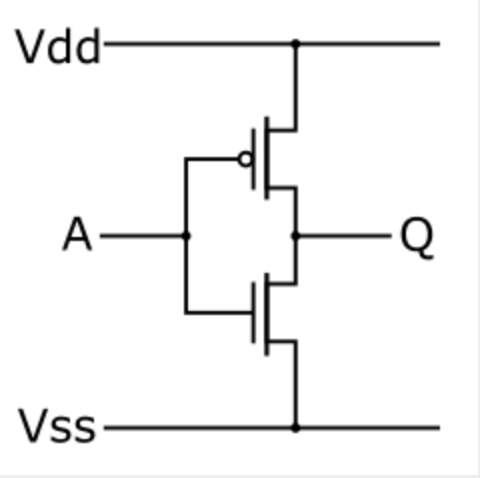
\includegraphics[width=0.8\textwidth]{assets/not.png}
    \caption{CMOSトランジスタを用いたNOTゲートの回路図}
    \label{fig:not_gate}
  \end{minipage}
  \hfill
  \begin{minipage}{0.45\textwidth}
    \centering
    \captionof{table}{NOTゲートの真理値表}
    \label{tab:not_truth_table}
    \begin{tabular}{|c|c|}
      \hline
      入力A & 出力Y \\ \hline
      0     & 1     \\ \hline
      1     & 0     \\ \hline
    \end{tabular}
  \end{minipage}
\end{figure}

\subsection{NANDゲート}
NANDゲートは、ANDゲートの出力を反転させたものである。両方の入力がHIGH閾値以上のときのみ出力がLOWとなる。

\begin{equation}
  Y = \overline{A \cdot B}
\end{equation}

\begin{figure}[H]
  \centering
  \begin{minipage}{0.45\textwidth}
    \centering
    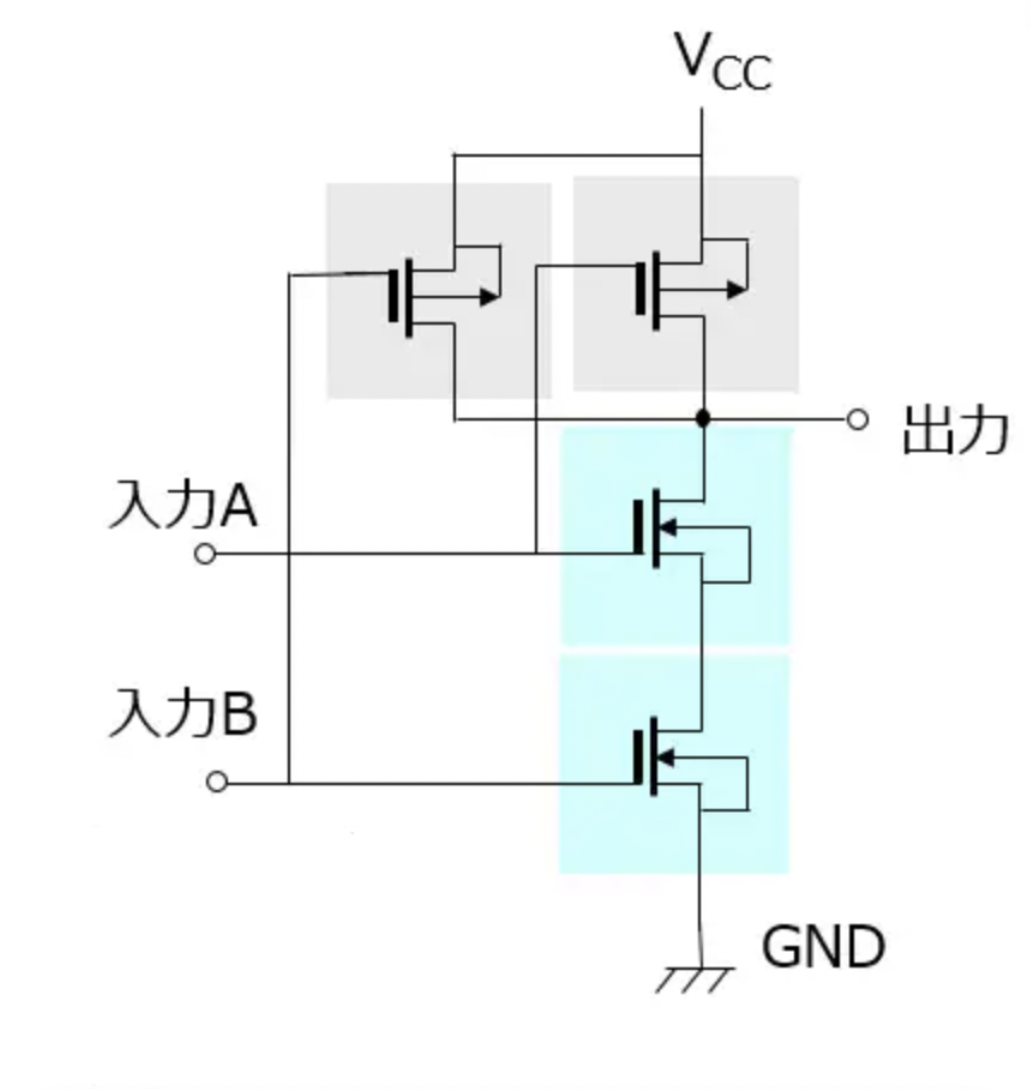
\includegraphics[width=0.8\textwidth]{assets/nand.png}
    \caption{CMOSトランジスタを用いたNANDゲートの回路図}
    \label{fig:nand_gate}
  \end{minipage}
  \hfill
  \begin{minipage}{0.45\textwidth}
    \centering
    \captionof{table}{NANDゲートの真理値表}
    \label{tab:nand_truth_table}
    \begin{tabular}{|c|c|c|}
      \hline
      入力A & 入力B & 出力Y \\ \hline
      0     & 0     & 1     \\ \hline
      0     & 1     & 1     \\ \hline
      1     & 0     & 1     \\ \hline
      1     & 1     & 0     \\ \hline
    \end{tabular}
  \end{minipage}
\end{figure}

\subsection{NORゲート}
NORゲートは、ORゲートの出力を反転させたものである。両方の入力がLOW閾値未満のときのみ出力がHIGHとなる。
\begin{equation}
  Y = \overline{A + B} 
\end{equation}

\begin{figure}[H]
  \centering
  \begin{minipage}{0.45\textwidth}
    \centering
    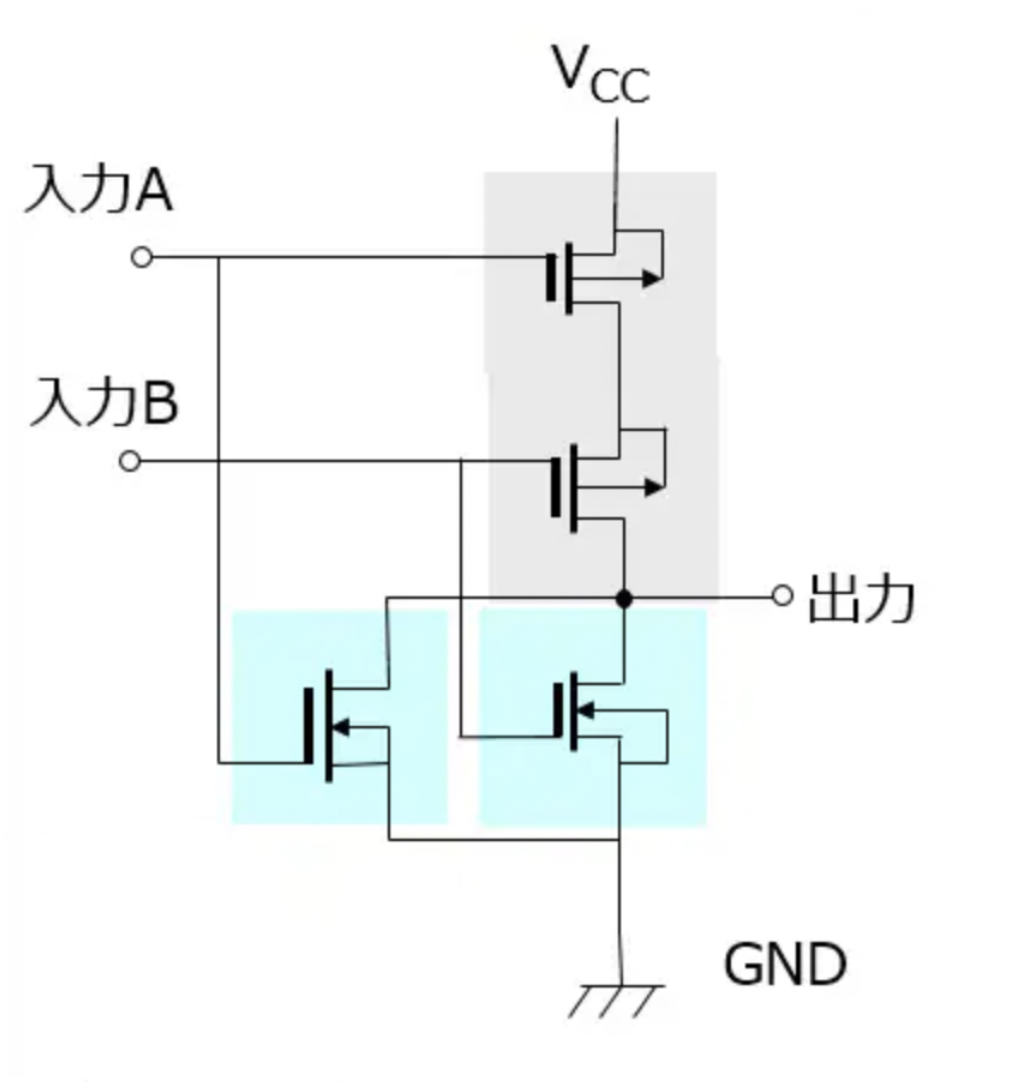
\includegraphics[width=0.8\textwidth]{assets/nor.png}
    \caption{CMOSトランジスタを用いたNORゲートの回路図}
    \label{fig:nor_gate}
  \end{minipage}
  \hfill
  \begin{minipage}{0.45\textwidth}
    \centering
    \captionof{table}{NORゲートの真理値表}
    \label{tab:nor_truth_table}
    \begin{tabular}{|c|c|c|}
      \hline
      入力A & 入力B & 出力Y \\ \hline
      0     & 0     & 1     \\ \hline
      0     & 1     & 0     \\ \hline
      1     & 0     & 0     \\ \hline
      1     & 1     & 0     \\ \hline
    \end{tabular}
  \end{minipage}
\end{figure}

\subsection{JK-FF}
JK-FFは、2つの入力信号JとKを持つフリップフロップである。クロック信号により状態が変化し、JとKの値に応じて出力Qが変化する。特に、立ち下がりエッジで出力が変化する。
\begin{equation}
  Q_{next} = J \cdot \overline{Q} + \overline{K} \cdot Q
\end{equation}

\begin{figure}[H]
  \centering
  \begin{minipage}{0.45\textwidth}
    \centering
    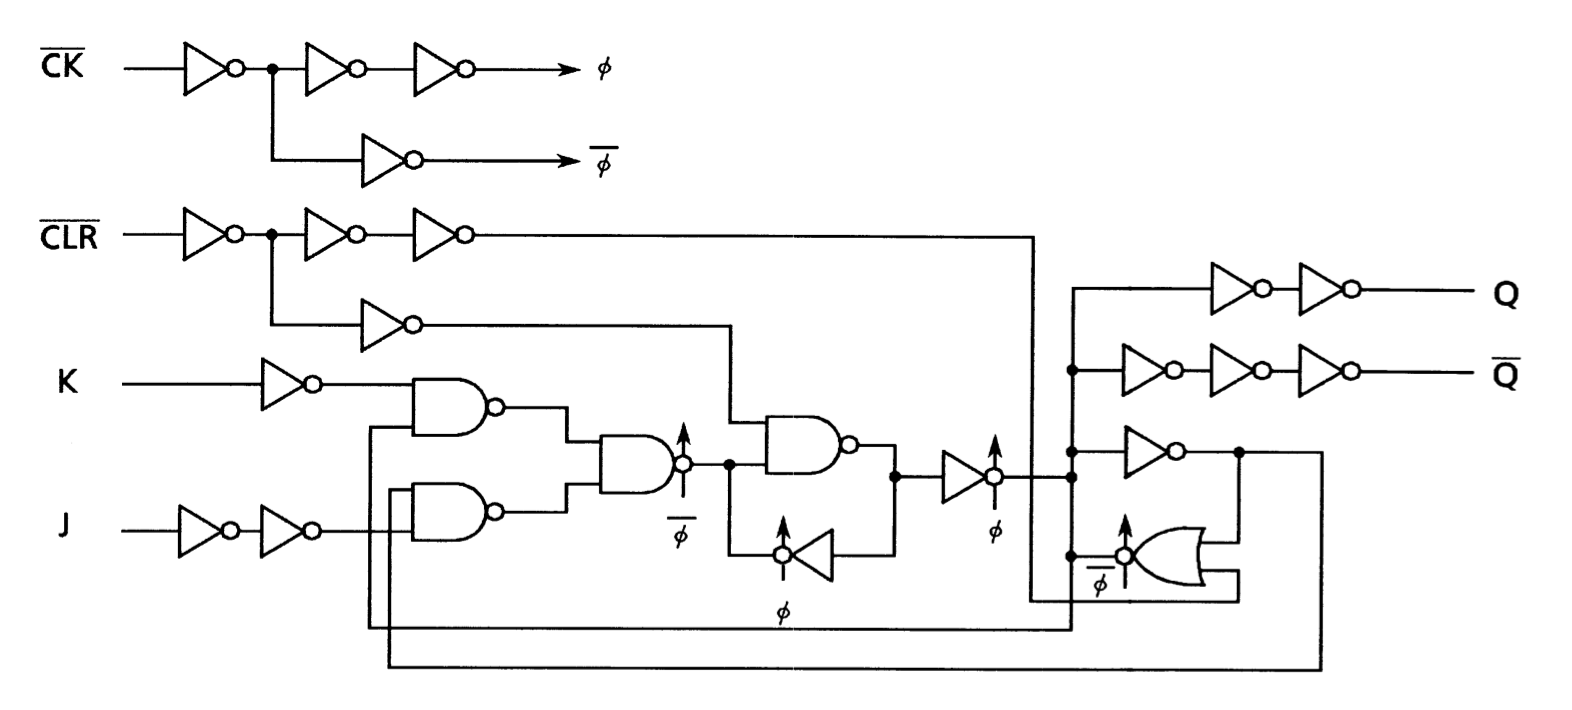
\includegraphics[width=1.2\textwidth]{assets/jk-ff.png}
    \caption{JK-FF(74HC107)の回路図}
  \end{minipage}
  \hfill
  \begin{minipage}{0.45\textwidth}
    \centering
      \captionof{table}{JK-FFの真理値表}
      \label{tab:jk_ff_truth_table}
      \begin{tabular}{|c|c|c|c|}
        \hline
        初期状態Q & J & K & 次状態Q(t+1) \\ \hline
        0 & 0 & 0 & 0 \\ \hline
        0 & 0 & 1 & 0 \\ \hline
        0 & 1 & 0 & 1 \\ \hline
        0 & 1 & 1 & 1 \\ \hline
        1 & 0 & 0 & 1 \\ \hline
        1 & 0 & 1 & 0 \\ \hline
        1 & 1 & 0 & 1 \\ \hline
        1 & 1 & 1 & 0 \\ \hline
      \end{tabular}
  \end{minipage}
\end{figure}

クロックが立ち上がりエッジのときに、JとKの値に応じて出力Qが変化する。JとKが両方ともHIGHの場合、出力は反転する。JがHIGHでKがLOWの場合、出力はHIGHになり、JがLOWでKがHIGHの場合、出力はLOWになる。

\subsection{D-FF}
D-FFは、1つのデータ入力Dを持つフリップフロップである。クロック信号によりDの値が出力Qに転送される。JK-FFを用いてD-FFを構成できる。
\begin{equation}
  Q_{next} = D
\end{equation}
\begin{figure}[H]
  \centering
  \begin{minipage}{0.45\textwidth}
    \centering
    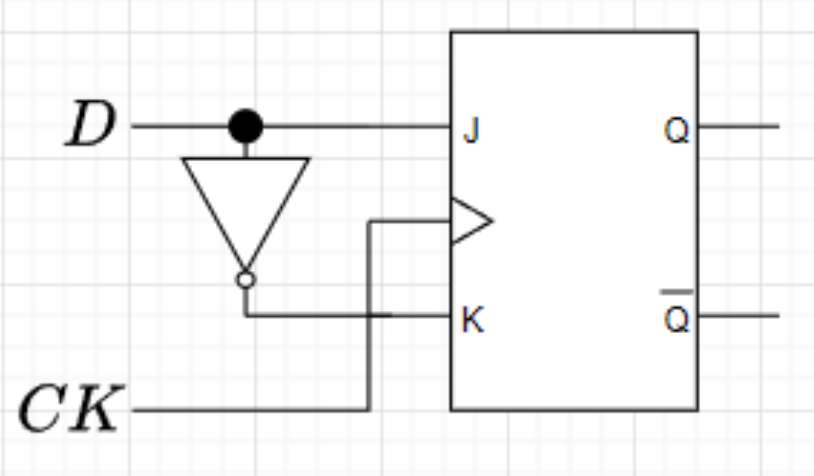
\includegraphics[width=0.8\textwidth]{assets/d-ff.png}
    \caption{D-FF(JK-FFとNOTで)の回路図}
  \end{minipage}
  \hfill
  \begin{minipage}{0.45\textwidth}
    \centering
      \captionof{table}{D-FFの真理値表}
      \label{tab:d_ff_truth_table}
      \begin{tabular}{|c|c|c|c|}
        \hline
        CK & D & Q & $\overline{Q}$ \\ \hline
        $\uparrow$ & 0 & 0 & 1 \\ \hline
        $\uparrow$ & 1 & 1 & 0 \\ \hline
      \end{tabular}
  \end{minipage}
\end{figure}
D-FFは、クロック信号の立ち上がりエッジでDの値を出力Qに転送する。クロック信号がLOWのとき、出力は前回の状態を保持する。

\subsection{シュミットトリガについて}
シュミットトリガは、入力信号の変化に対して出力信号が遅延する特性を持つ。これにより、ノイズに強く、安定した動作が可能となる。また、入力信号の上昇エッジと下降エッジで異なる閾値を持つため、ヒステリシス効果を利用しスイッチングの安定性を高めている。

\section{実験手順}
\subsection{ド・モルガンの法則の確認}
\begin{enumerate}
  \item ベン図での確認
  \item 真理値表での確認
  \item 論理回路での確認 \\
  - NOTゲートとNANDゲートを使用した場合 \\
  - NOTゲートとNORゲートを使用した場合
  \item 半加算器(HA) \\
  - 図3.1の回路の真理値表を完成させる。 \\
  - 図3.1の回路をNANDゲートとNOTゲートのみを用いて設計し、設計した回路の真理値表が同様であることを確認する。
\end{enumerate}

\begin{figure}[H]
  \centering
  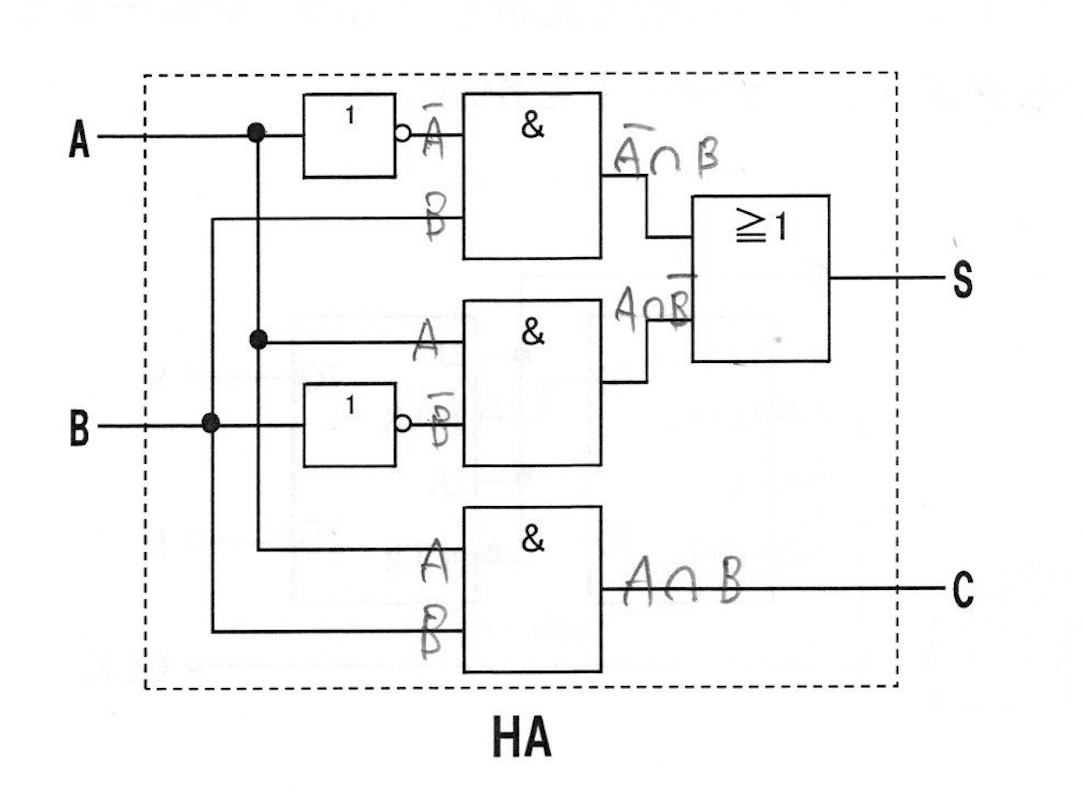
\includegraphics[width=0.6\textwidth]{assets/HAkairo.png}
  \caption{半加算器(HA)の回路図}
\end{figure}

\subsection{信号発声器の設計と製作}
図3.2の回路の各部をオシロスコープで測定し、A点, CLK, 1Q, \(\overline{\text{1Q}}\), S, Rのタイミングチャートを作成する。

\begin{figure}[H]
  \centering
  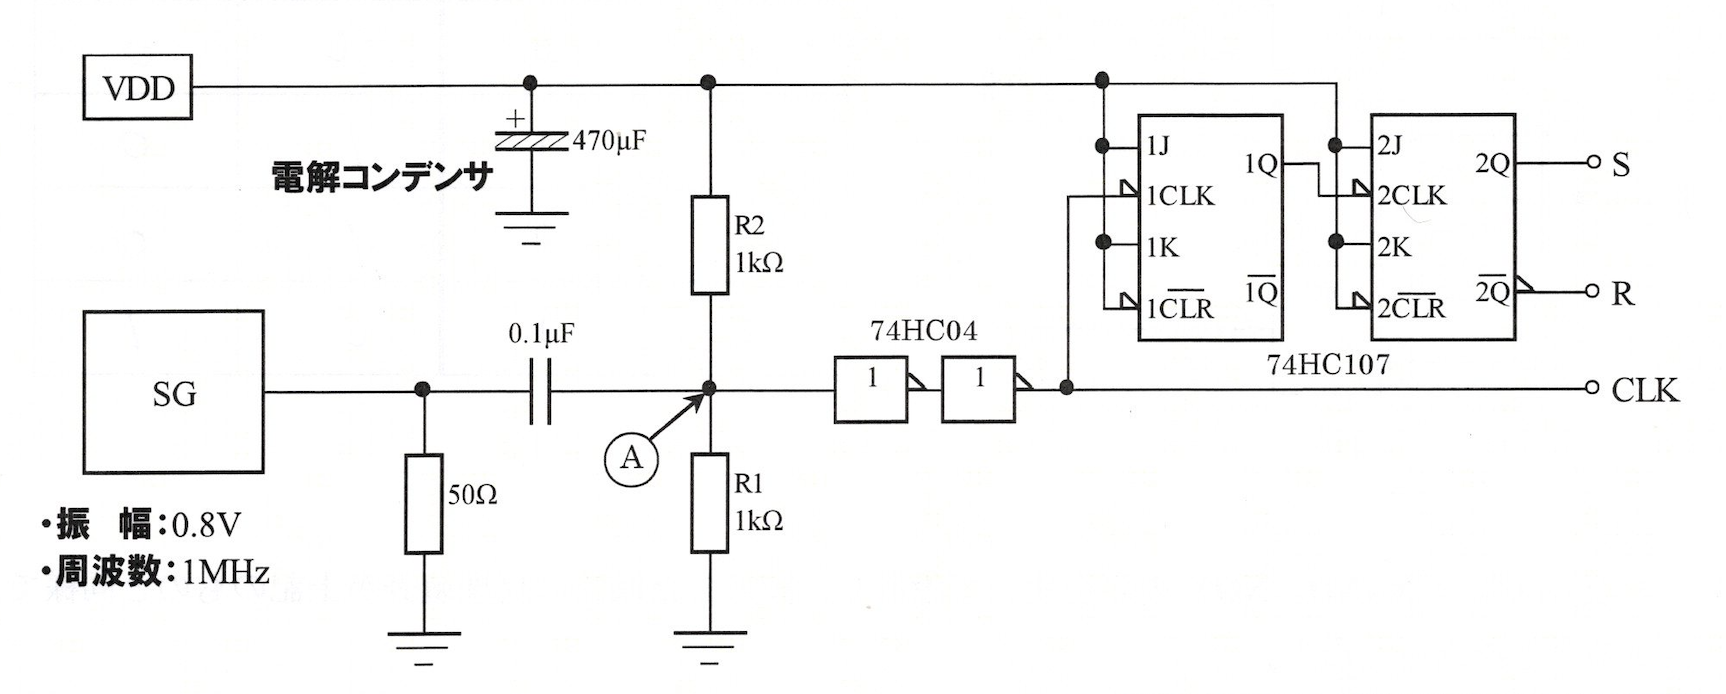
\includegraphics[width=\textwidth]{assets/SGkairo.png}
  \caption{信号発生器の回路図}
\end{figure}

\subsection{同期式SR-FFの動作と特性}
図3.3の回路を制作し、CLK,S,R,a,b,Q,\(\overline{Q}\)のタイミングチャートを作成する。

\begin{figure}[H]
  \centering
  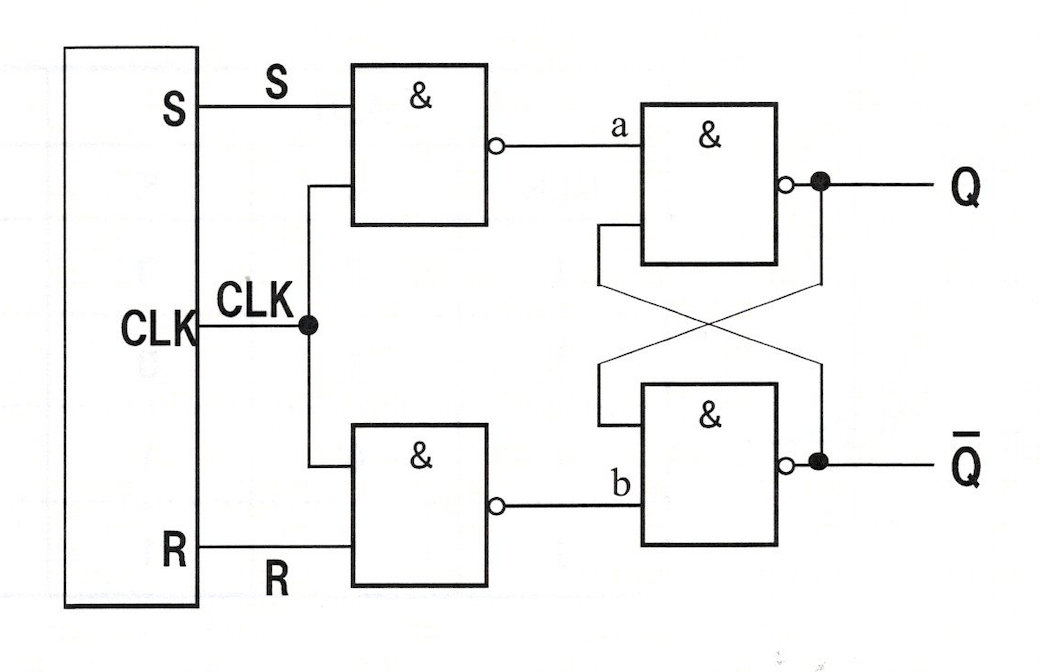
\includegraphics[width=0.6\textwidth]{assets/srffkairo.png}
  \caption{同期式SR-FFの回路図}
\end{figure}

\subsection{JK-FFの動作と特性}
図3.4の回路を制作し、CLK,S,1Qのタイミングチャートを作成する。

\begin{figure}[H]
  \centering
  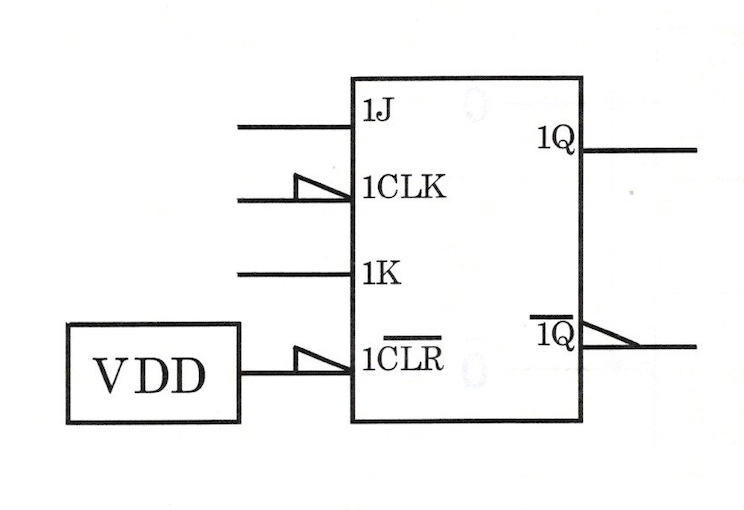
\includegraphics[width=0.6\textwidth]{assets/jkffkairo.png}
  \caption{JK-FFの回路図}
\end{figure}

\subsection{D-FFの動作と特性}
\begin{enumerate}
  \item D-FFの真理値表を完成させる。
  \item JK-FFとNOTゲートを用いてD-FFを構成する。
  \item 2.で構成した回路を制作し、CLK,D,Q,\(\overline{Q}\)のタイミングチャートを作成する。
\end{enumerate}

\subsection{カウンタの設計}
\subsubsection{非同期式1/3カウンタ}
図3.5の回路を制作し、CLK,1J,\(Q_0\),\(Q_1\)のタイミングチャートを作成する。

\begin{figure}[H]
  \centering
  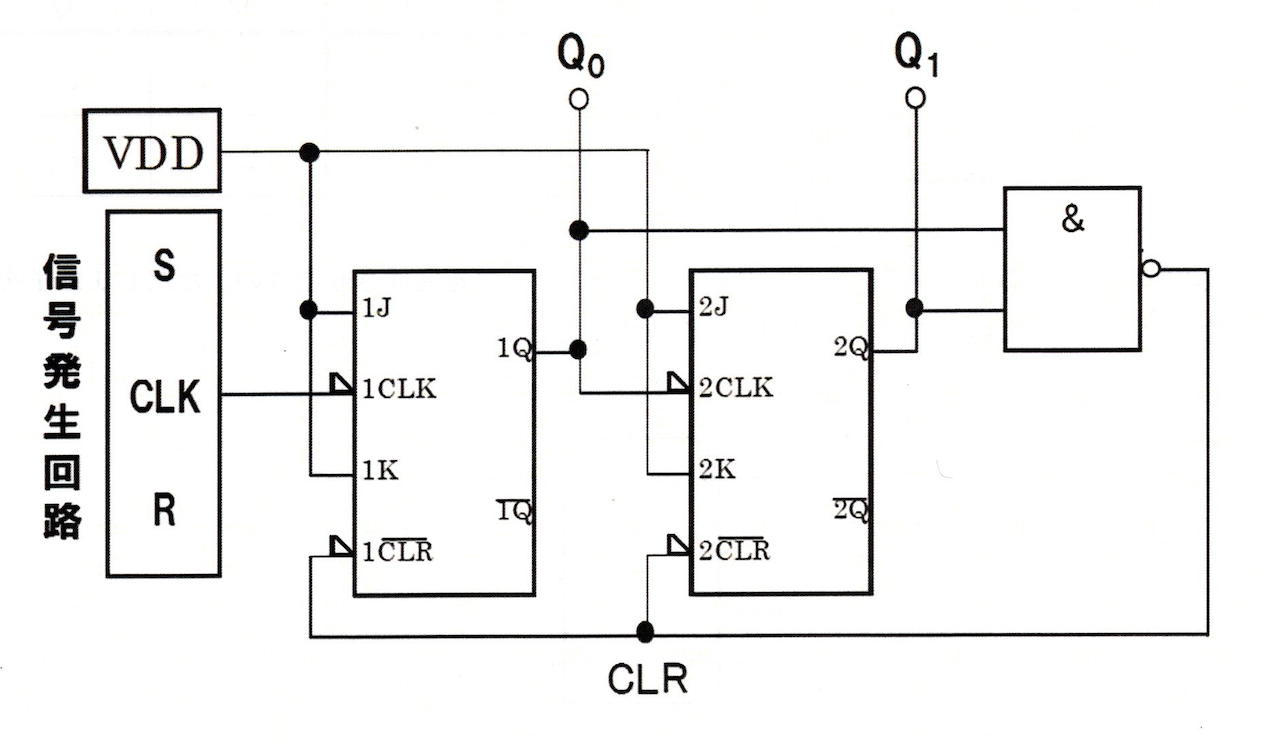
\includegraphics[width=0.6\textwidth]{assets/hidoukicounter.png}
  \caption{非同期式1/3カウンタの回路図}
\end{figure}

\subsubsection{同期式1/3カウンタ}
図3.6の回路を制作し、CLK,1J,\(Q_0\),\(Q_1\)のタイミングチャートを作成する。

\begin{figure}[H]
  \centering
  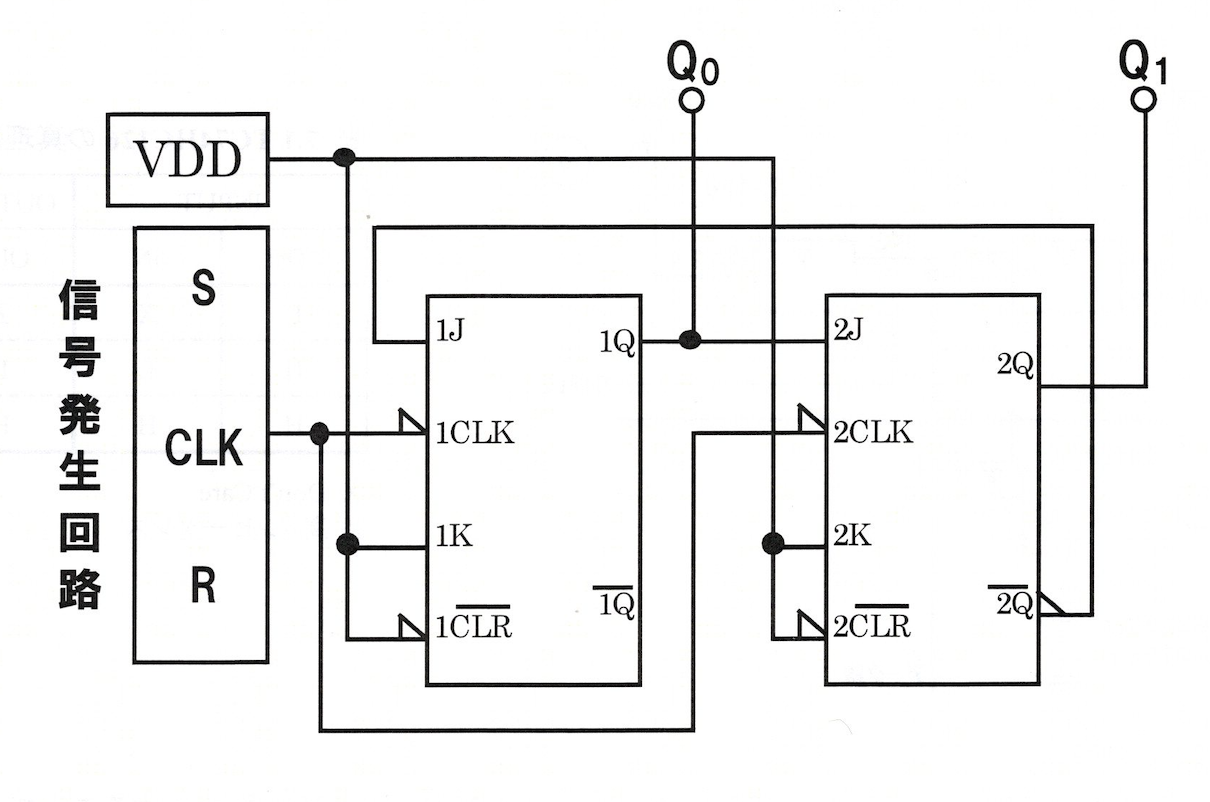
\includegraphics[width=0.6\textwidth]{assets/doukicounter.png}
  \caption{同期式1/3カウンタの回路図}
\end{figure}

\subsection{メモリ機能}
図3.7の回路を作成し、表3.1の操作をしたときの結果を測定する。なお、1は5V電位、0はGND電位とする。

\begin{figure}[H]
  \centering
  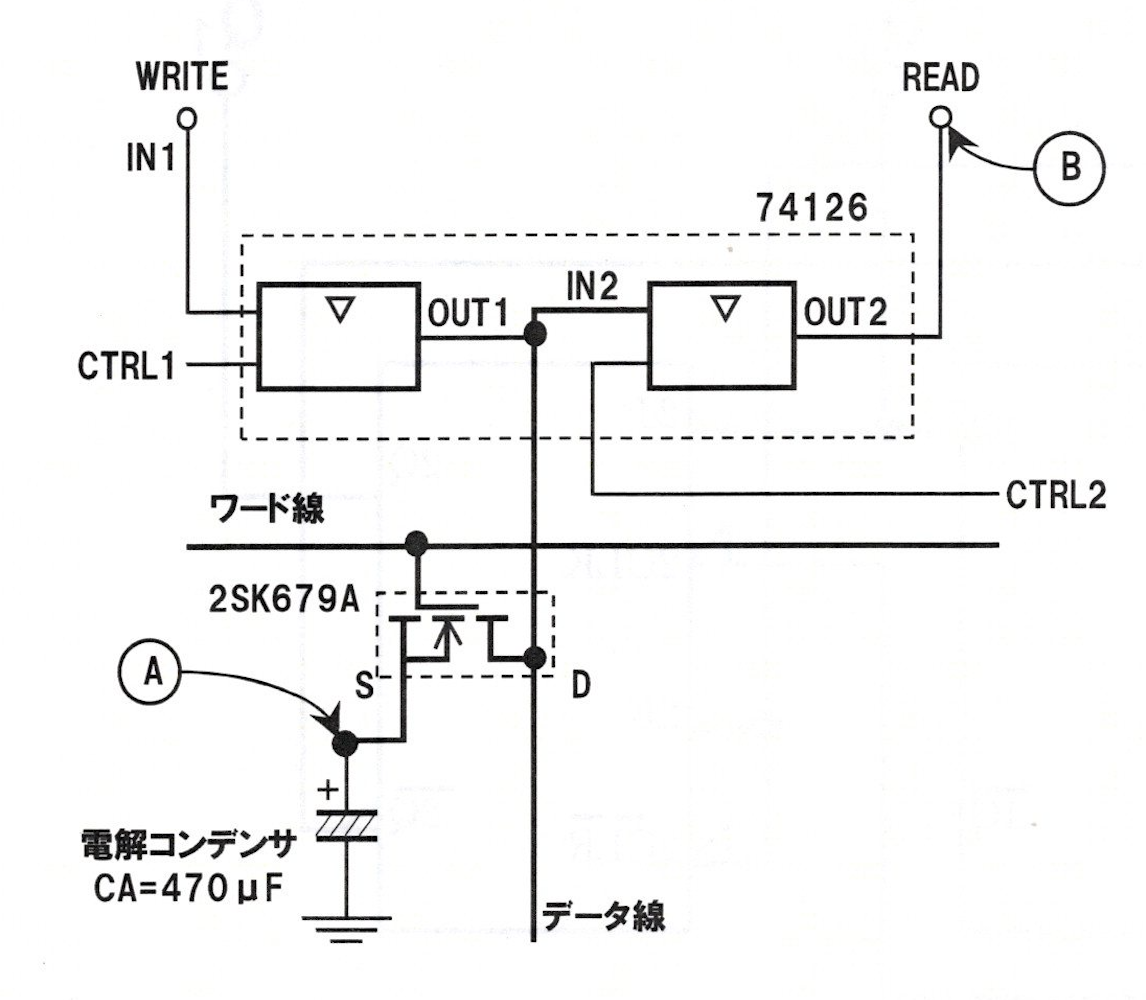
\includegraphics[width=0.6\textwidth]{assets/memorykairo.png}
  \caption{DRAMのリード・ライト回路図}
\end{figure}

\begin{table}[H]
  \centering
  \caption{DRAMの書き込みと読み出しの手順}
  \begin{tabular}{c}
    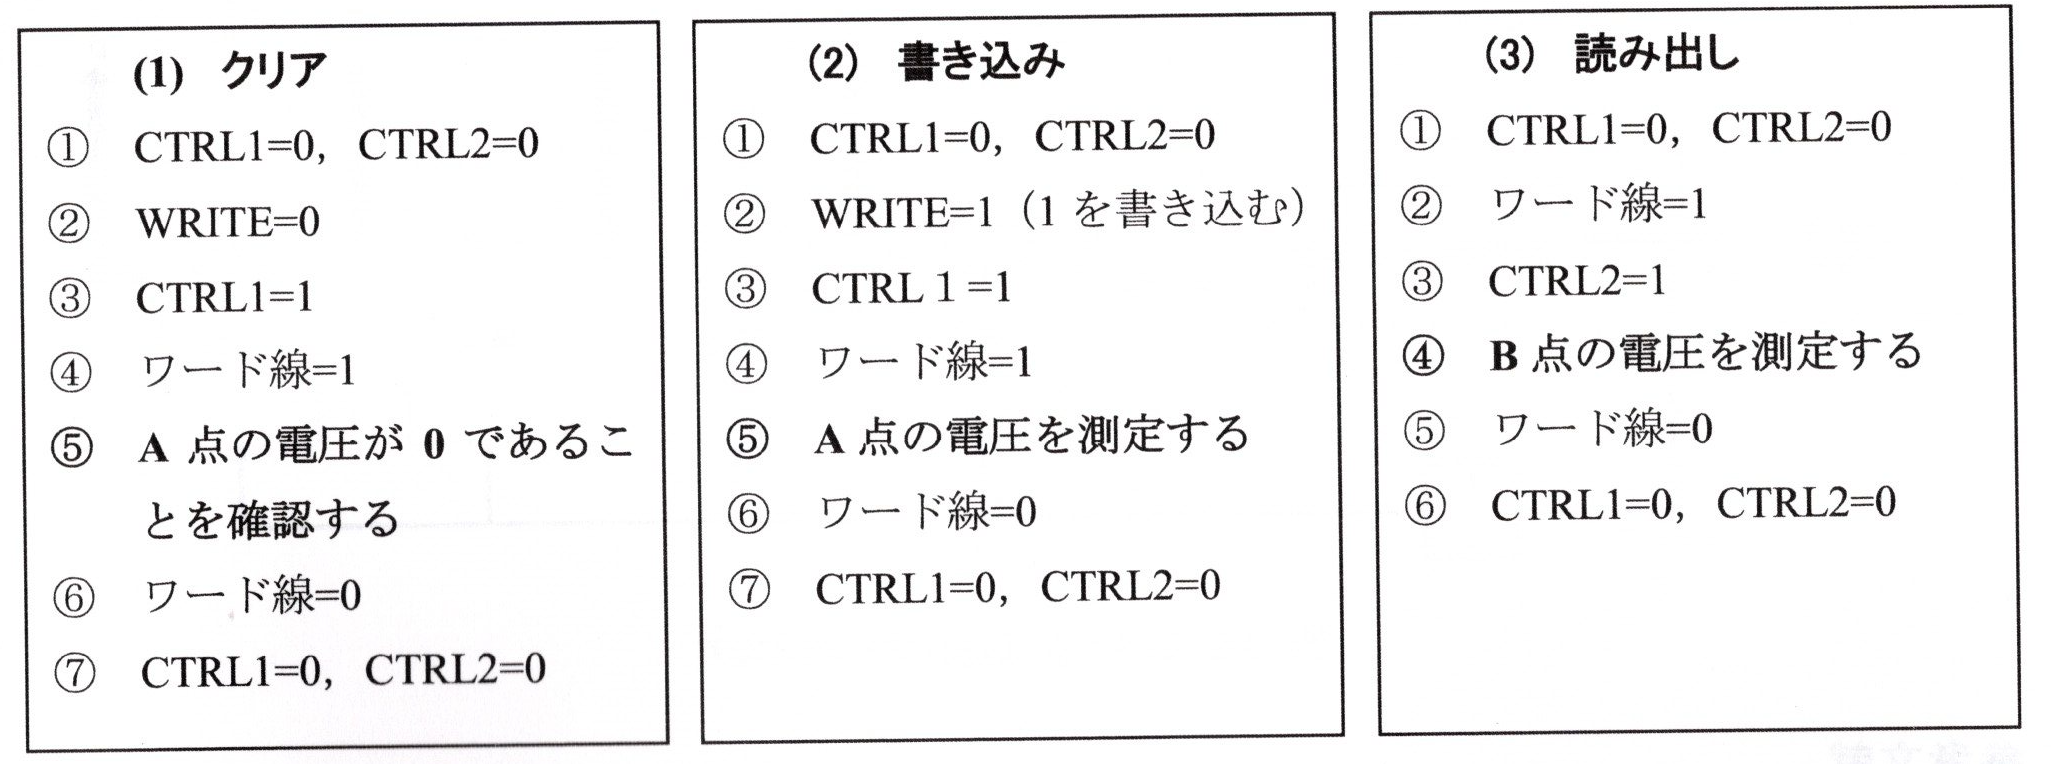
\includegraphics[width=0.8\textwidth]{assets/memoryctrl.png} \\
  \end{tabular}
\end{table}

\begin{enumerate}
  \item WRITE=0, CTRL=1, ワード線=1 にすることで2SK679Aはどのような状態になるか
  \item WRITE=1, CTRL=1, ワード線=1 にすることで2SK679Aはどのような状態になるか
  \item 呼び出し操作をした際のB点の電圧はいくらになるか
\end{enumerate}

\section{実験結果}
\subsection{ド・モルガンの法則の確認}
\subsubsection{ベン図での確認}
図4.1に示す。

\begin{figure}[H]
  \centering
  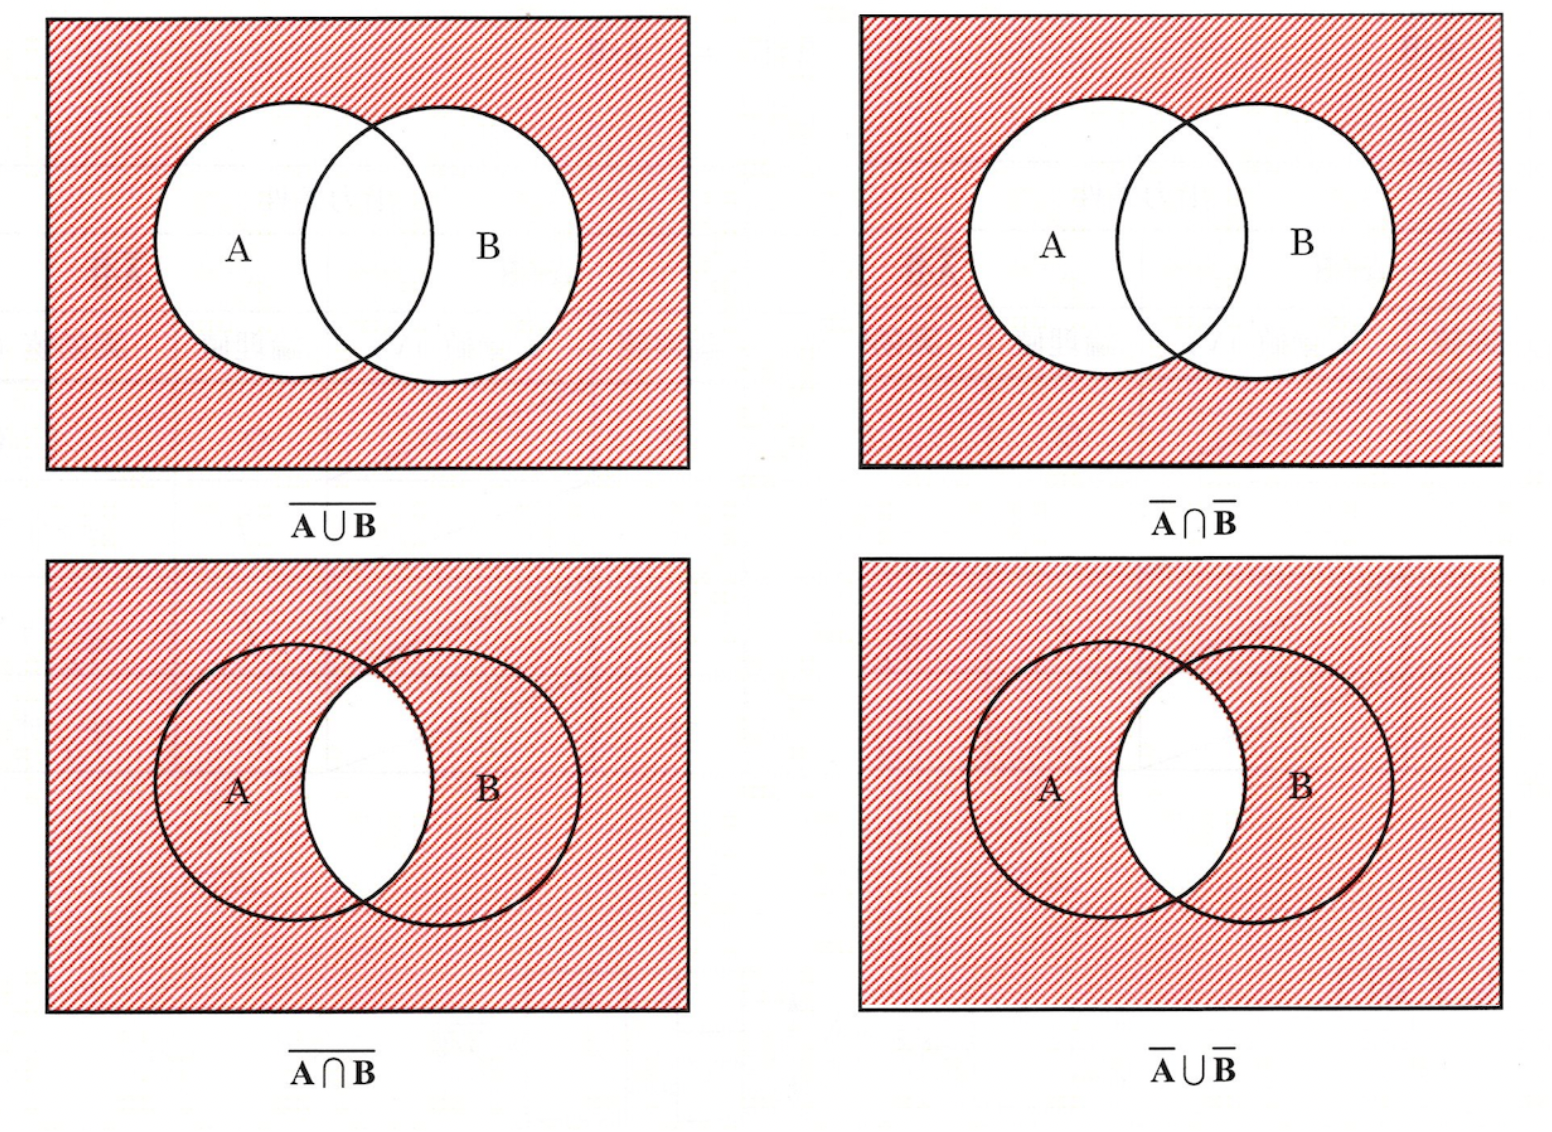
\includegraphics[width=0.6\textwidth]{assets/benzu.png}
  \caption{ベン図}
\end{figure}

\subsubsection{真理値表での確認}
4.1.1で作成したベン図をもとに、ある要素xが集合AまたはBに属しているとき○、属していないとき×で表したものを、表4.1に示す。

\begin{table}[H]
  \centering
  \caption{真理値表}
  \begin{tabular}{c}
    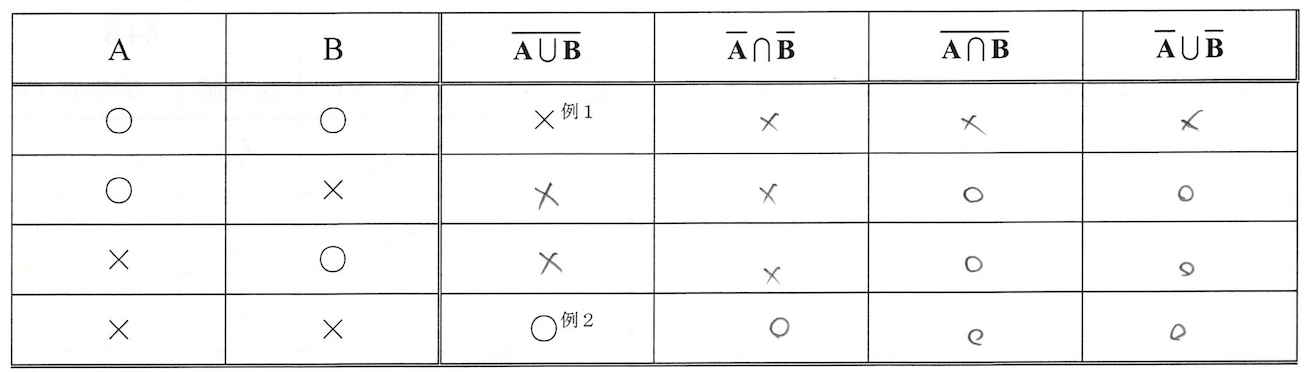
\includegraphics[width=0.8\textwidth]{assets/domoshinri.png} \\
  \end{tabular}
\end{table}

\subsubsection{論理回路での確認}
\begin{enumerate}
  \item NOTゲートとNANDゲートを使用した場合、図4.2のように変換でき、その回路を制作し測定した結果を表4.2に示す。
  
  \begin{figure}[H]
  \centering
  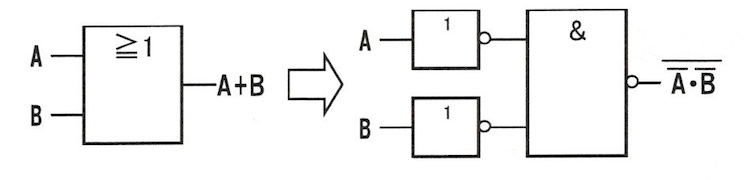
\includegraphics[width=0.6\textwidth]{assets/notnand.png}
  \caption{NOTゲートとNANDゲートを使用した場合}
  \end{figure}

  \begin{table}[H]
  \centering
  \caption{入力条件と出力条件の各種値}
  \begin{tabular}{c}
    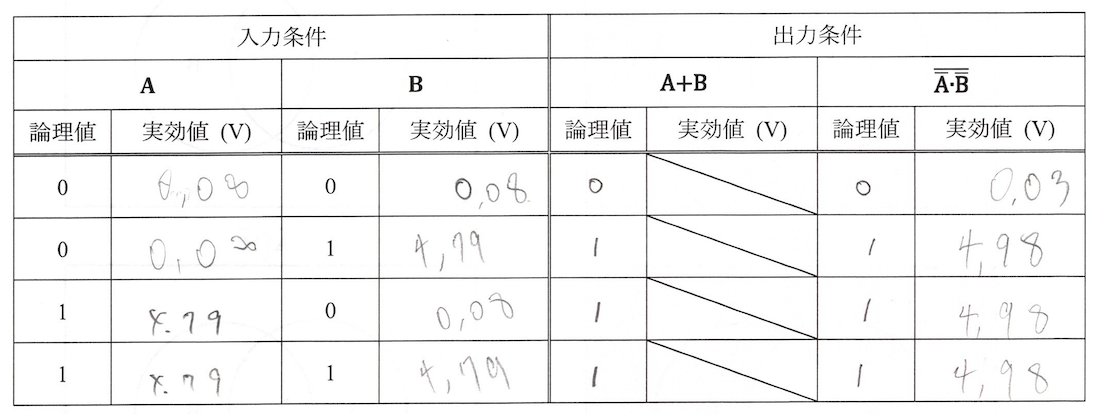
\includegraphics[width=0.8\textwidth]{assets/notnandshinri.png} \\
  \end{tabular}
  \end{table}

  \item NOTゲートとNORゲートを使用した場合、図4.3のように変換でき、その回路を制作し測定した結果を表4.3に示す。
  
  \begin{figure}[H]
  \centering
  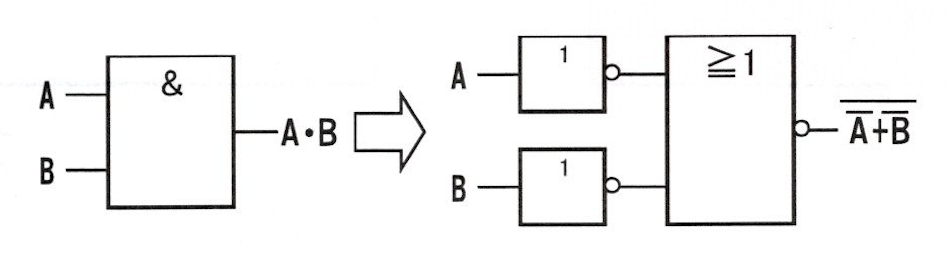
\includegraphics[width=0.6\textwidth]{assets/notnor.png}
  \caption{NOTゲートとNORゲートを使用した場合}
  \end{figure}

  \begin{table}[H]
  \centering
  \caption{入力条件と出力条件の各種値}
  \begin{tabular}{c}
    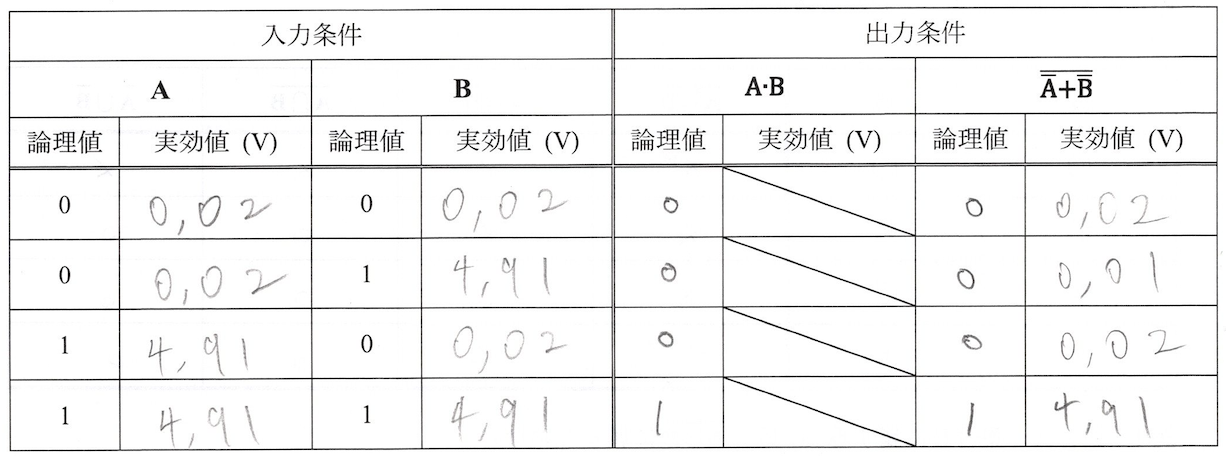
\includegraphics[width=0.8\textwidth]{assets/notnorshinri.png} \\
  \end{tabular}
  \end{table}

\end{enumerate}

\subsubsection{半加算器(HA)の設計}
図3.1の回路の真理値表を表4.4に示す。

\begin{table}[H]
  \centering
  \caption{半加算器(HA)の真理値表}
  \begin{tabular}{|c|c|c|c|}
    \hline
    A & B & S & C \\ \hline
    0 & 0 & 0 & 0 \\ \hline
    0 & 1 & 1 & 0 \\ \hline
    1 & 0 & 1 & 0 \\ \hline
    1 & 1 & 0 & 1 \\ \hline
  \end{tabular}
\end{table}

また、図3.2の回路をNANDゲートとNOTゲートのみを用いて設計すると、図4.4のようになる。

\begin{figure}[H]
  \centering
  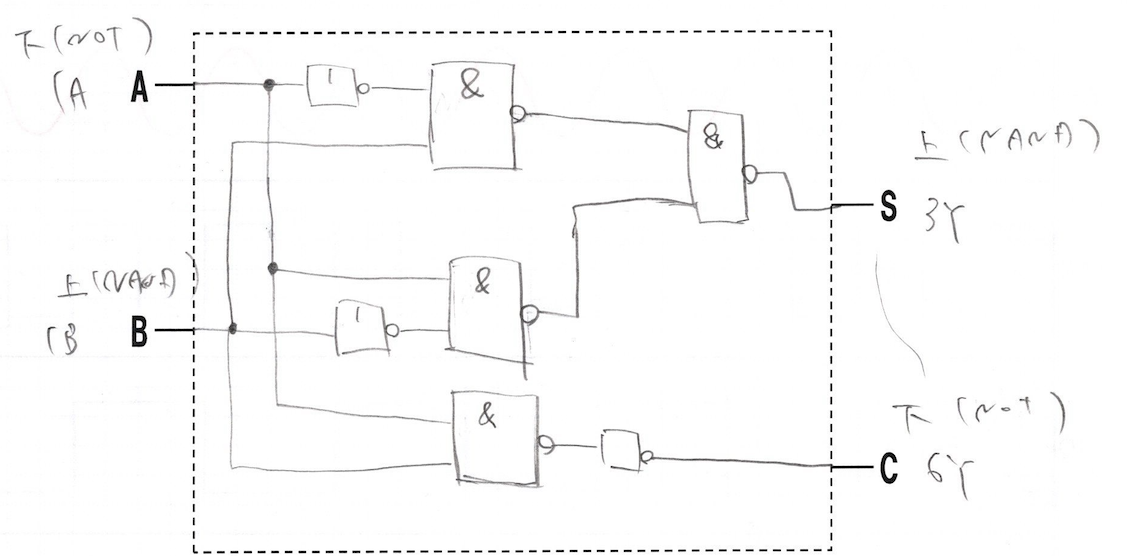
\includegraphics[width=0.6\textwidth]{assets/hanandnot.png}
  \caption{NANDゲートとNOTゲートを使用した場合}
\end{figure}

図4.4の回路の真理地表は表4.5のようになり、表4.4と同様であることが確認できた。

\begin{table}[H]
  \centering
  \caption{図4.4の真理値表}
  \begin{tabular}{c}
    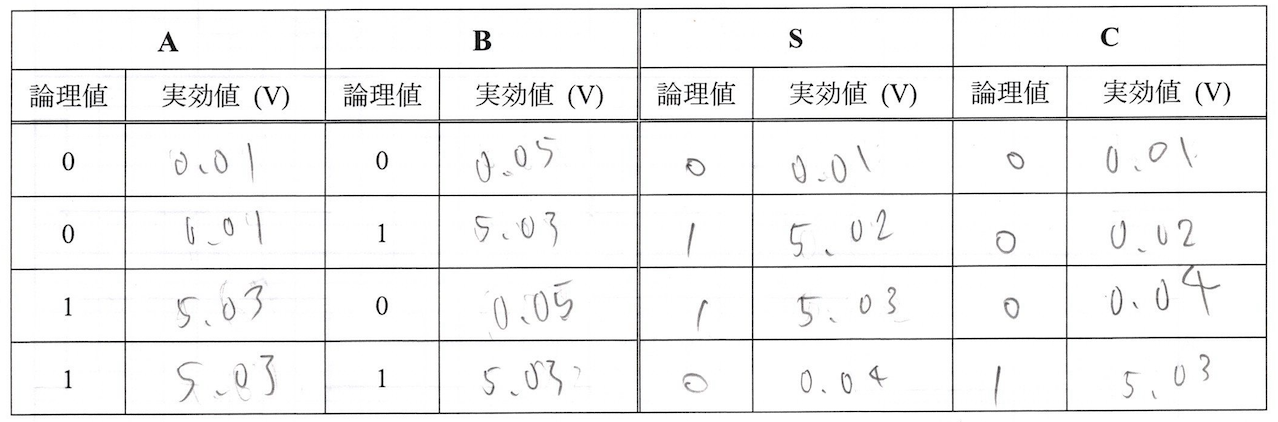
\includegraphics[width=0.8\textwidth]{assets/hanandnotshinri.png} \\
  \end{tabular}
\end{table}

\subsection{信号発生器の設計と製作}
図3.2の回路の各部のオスロスコープで観測した波形を図4.5(上から順にA 点、CLK、1Q、1Q)、4.6(上から順にA 点、S、R)に示す。

\begin{figure}[H]
  \centering
  \begin{minipage}{0.48\textwidth}
    \centering
    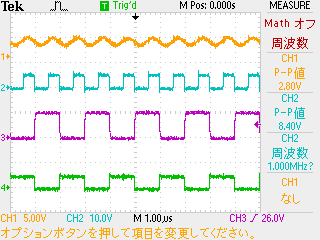
\includegraphics[width=\textwidth]{assets/sg01.png}
    \caption{A点、CLK、1Q、\(\overline{1Q}\)の観測波形}
  \end{minipage}
  \hfill
  \begin{minipage}{0.48\textwidth}
    \centering
    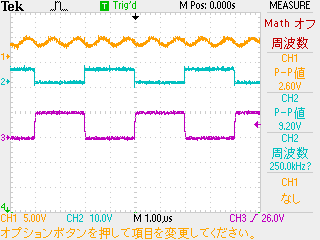
\includegraphics[width=\textwidth]{assets/sg02.png}
    \caption{A点、S、Rの観測波形}
  \end{minipage}
\end{figure}

また、図 4.5,4.6 のオシロスコープで観測波形より作成したタイミングチャートを図 4.7 に示す。

\begin{figure}[H]
  \centering
  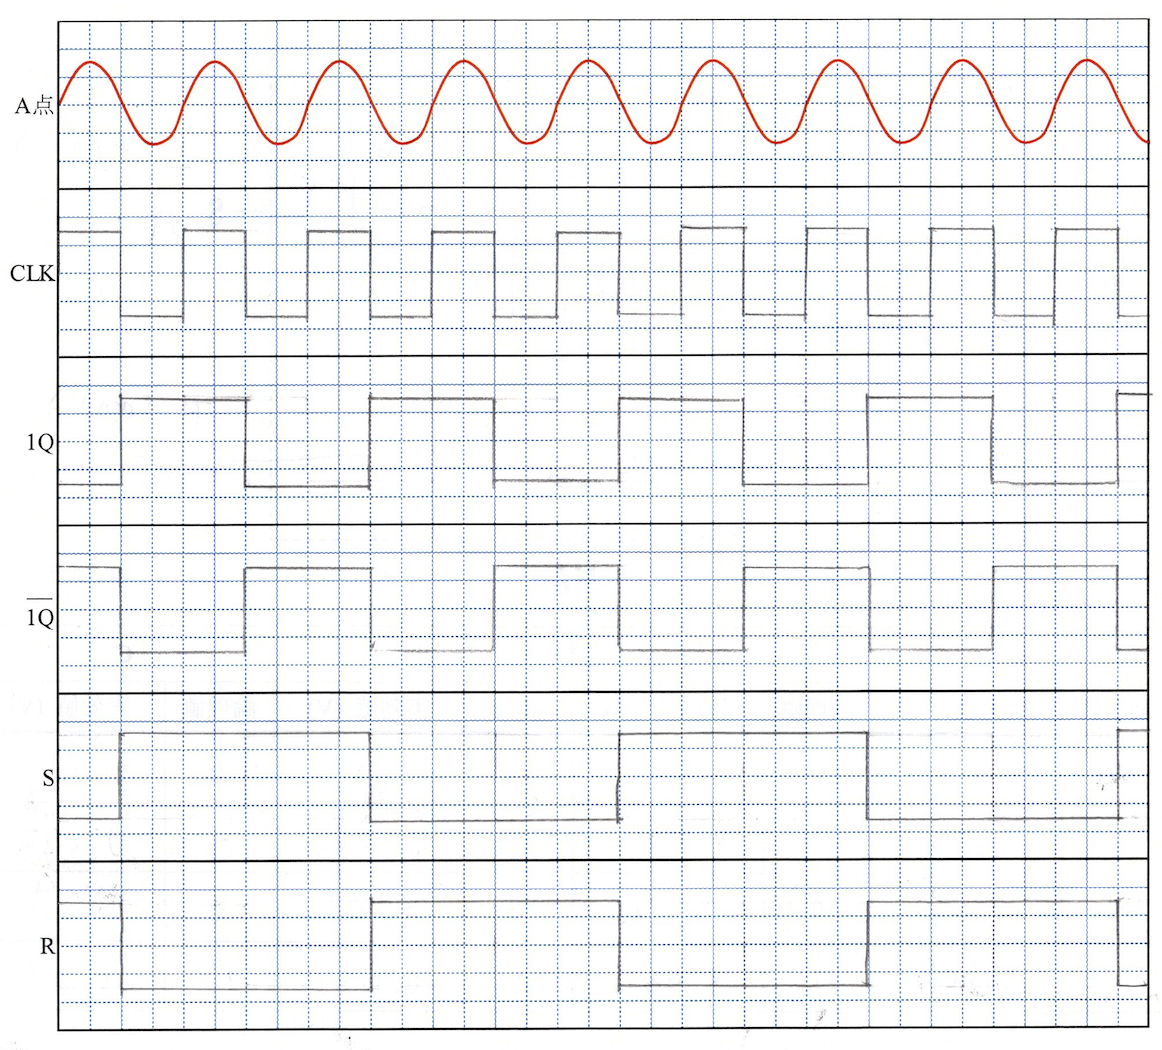
\includegraphics[width=0.8\textwidth]{assets/sgchart.png}
  \caption{信号発生器のタイミングチャート}
\end{figure}

図4.7より、A点での正弦波がCLK信号では矩形波として現れており、1Qで
はその矩形波の周期の2倍の矩形波が、\(\overline{1Q}\)ではそれが反転したものが、Sでは1Qの矩形波の周期がさらに2倍になった矩形波が、Rではそれが反転したものが現れていることが確認できた。

\subsection{同期式SR-FFの動作と特性}
図3.3の回路を制作し、各測定点(CLK, S, R, a, b, Q, \(\overline{Q}\))のオスロスコープで観測した波形を図4.8(上から順にCLK、S、R、a)、4.9(上から順にCLK、b、Q、Q)に示す。

\begin{figure}[H]
  \centering
  \begin{minipage}{0.48\textwidth}
    \centering
    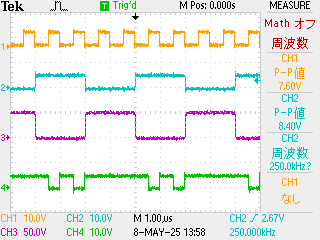
\includegraphics[width=\textwidth]{assets/srff01.png}
    \caption{CLK、S、R、aの観測波形}
  \end{minipage}
  \hfill
  \begin{minipage}{0.48\textwidth}
    \centering
    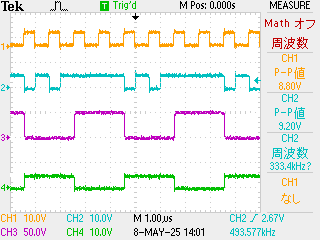
\includegraphics[width=\textwidth]{assets/srff02.png}
    \caption{CLK、b、Q、\(\overline{Q}\)の観測波形}
  \end{minipage}
\end{figure}

また、図 4.8,4.9 のオシロスコープでの観測波形より作成したタイミングチャートを図4.10 に示す。

\begin{figure}[H]
  \centering
  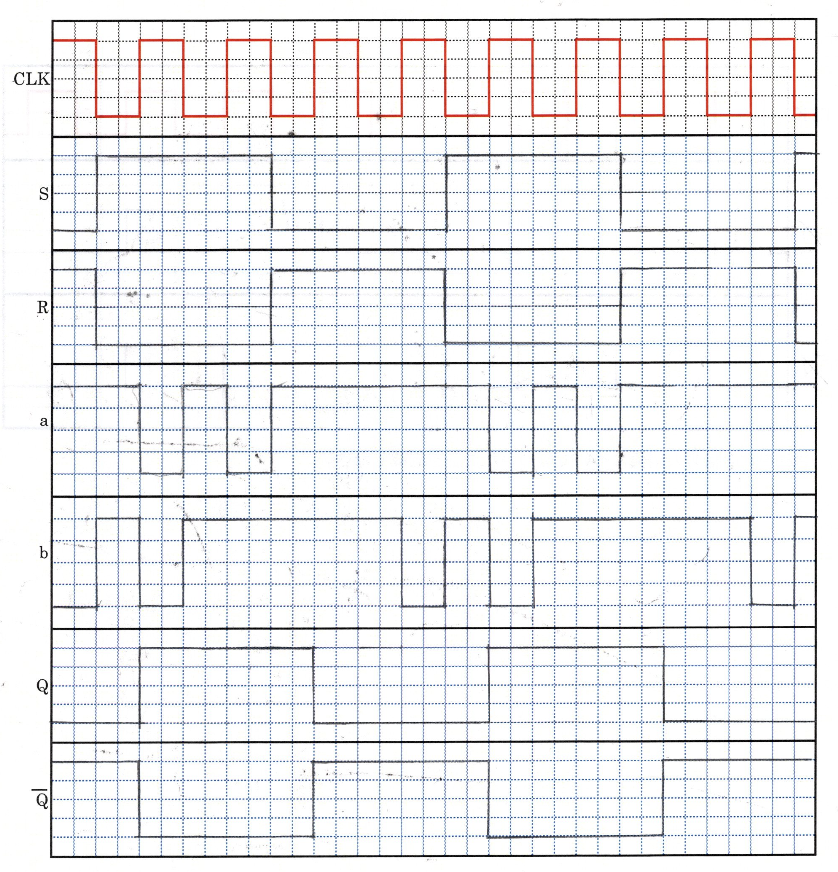
\includegraphics[width=0.8\textwidth]{assets/srffchart.png}
  \caption{同期式SR-FFのタイミングチャート}
\end{figure}

図4.10より、SではCLKの4倍の周期の矩形波が、Rではそれが反転したものが現れていることが確認できた。
また、Qでは位相がずれたCLKの4倍の周期の矩形波が現れ、\(\overline{Q}\)ではそれが反転したものが現れていることが確認できた。
さらに、aとbではS,Rの2倍周期で大きなものと小さなものの2種類がある矩形波が現れていることが確認できた。

\subsection{JK-FFの動作と特性}
図3.4の回路を制作し、各測定点(CLK, S, 1Q)のオスロスコープで観測した波形を図4.11に示す。

\begin{figure}[H]
  \centering
  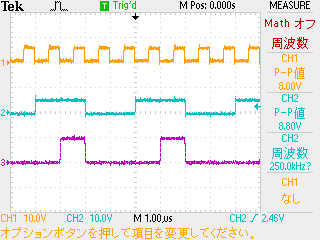
\includegraphics[width=0.4\textwidth]{assets/jkff.png}
  \caption{CLK、S、1Qの観測波形}
\end{figure}

また、図4.11のオシロスコープでの観測波形より作成したタイミングチャートを図4.12に示す。

\begin{figure}[H]
  \centering
  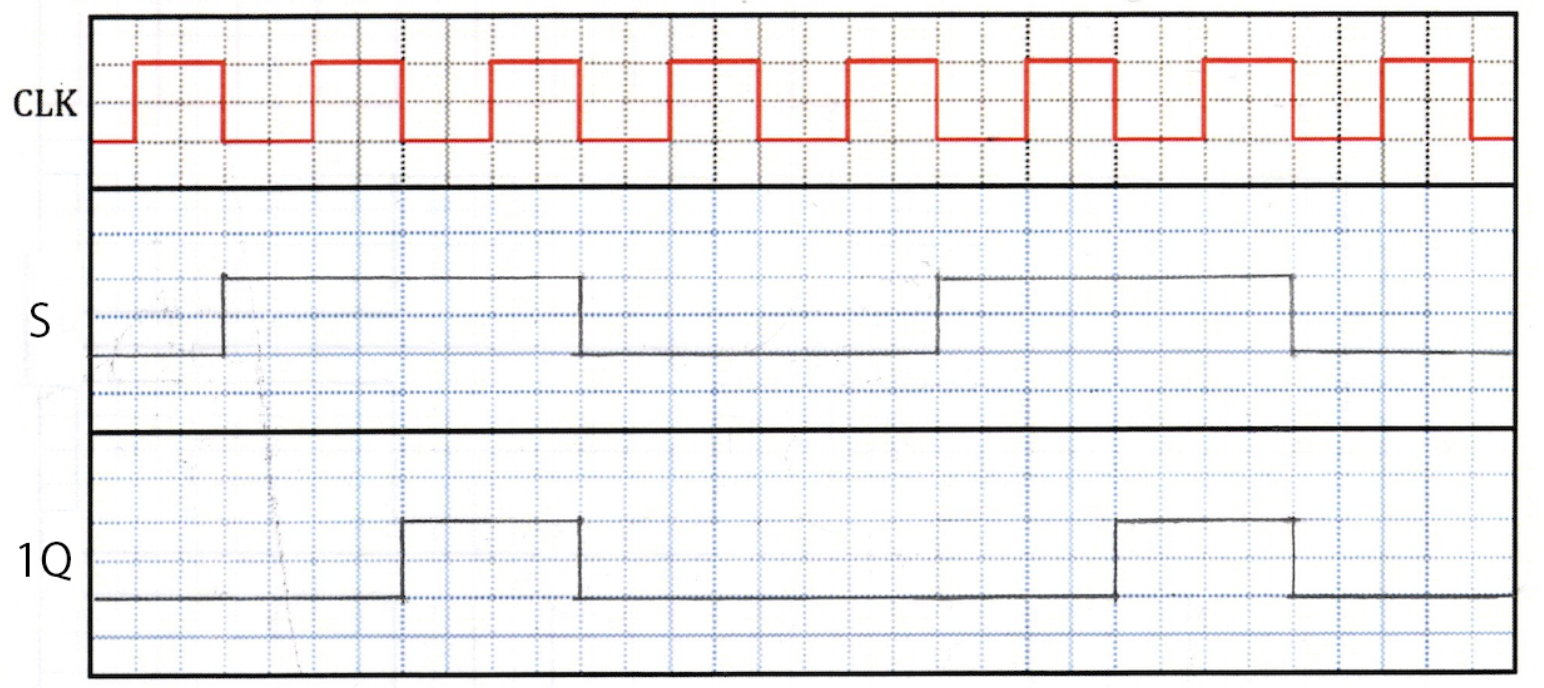
\includegraphics[width=0.8\textwidth]{assets/jkffchart.png}
  \caption{JK-FFのタイミングチャート}
\end{figure}

図4.12より、SではCLKの4倍の周期の矩形波が、1QではSがHIGHになった次のCLKの周期でHIGHになっていることが確認できた。

\subsection{D-FFの動作と特性}
\begin{enumerate}
  \item D-FFの真理値表を表4.6に示す。
  
  \begin{table}[H]
    \centering
    \caption{D-FFの真理値表}
    \begin{tabular}{|c|c|c|c|}
      \hline
      CLK & D & Q & $\overline{Q}$ \\ \hline
      $\downarrow$ & 1 & 1 & 0 \\ \hline
      $\downarrow$ & 0 & 0 & 1 \\ \hline
    \end{tabular}
  \end{table}

  \item JK-FFとNOTゲートを用いてD-FFを構成したものを図4.13に示す。
  
  \begin{figure}[H]
  \centering
  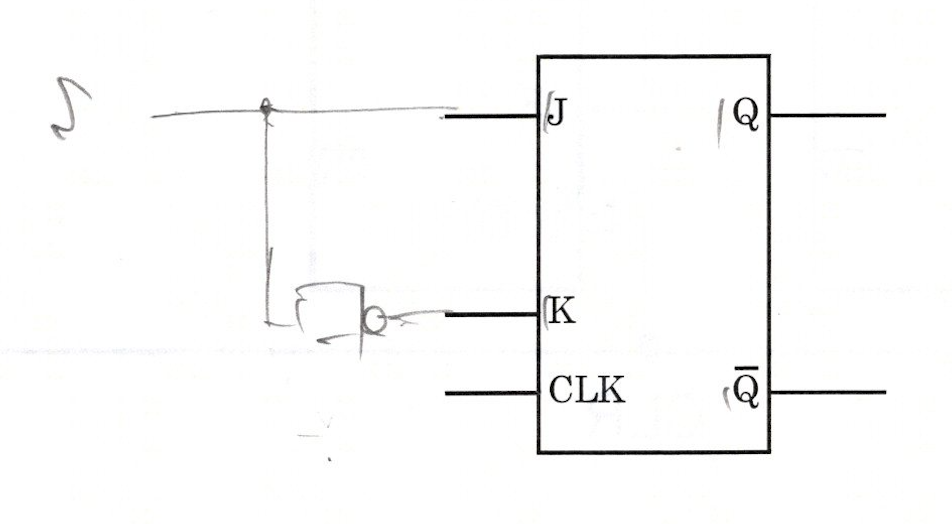
\includegraphics[width=0.6\textwidth]{assets/dffkairo.png}
  \caption{JK-FFとNOTゲートで構成したD-FFの回路図}
  \end{figure}

  \item 図4.10の回路を制作し、各測定点(CLK, D, Q, \(\overline{Q}\))のオスロスコープで観測した波形を図4.14(上から順にCLK、D、Q)に示す。
  
  \begin{figure}[H]
  \centering
  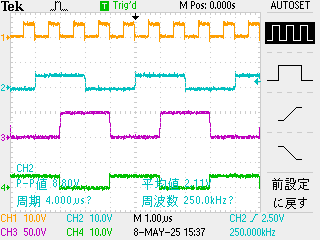
\includegraphics[width=0.4\textwidth]{assets/dff.png}
  \caption{CLK、D、Qの観測波形}
  \end{figure}

  また、図4.14のオシロスコープでの観測波形より作成したタイミングチャートを図4.15に示す。
  \begin{figure}[H]
  \centering
  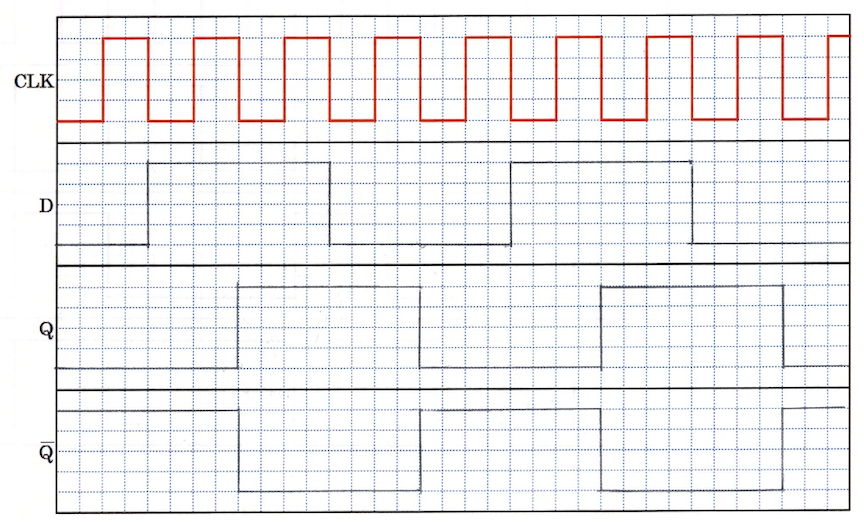
\includegraphics[width=0.8\textwidth]{assets/dffchart.png}
  \caption{D-FFのタイミングチャート}
  \end{figure}

  図4.15より、DではCLKの4倍の周期の矩形波が現れ、Qでは位相がDと1/4周期遅れた矩形波が現れ、\(\overline{Q}\)ではそれが反転したものが現れていることが確認できた。
\end{enumerate}

\subsection{カウンタの設計}
\subsubsection{非同期式1/3カウンタ}
図3.6の回路の各測定点(CLK、\(Q_0\)、\(Q_1\)、CLR)のオスロスコープで観測した波形を図4.12(上から順にCLK、Q0、Q1、CLR)に示す。

\begin{figure}[H]
  \centering
  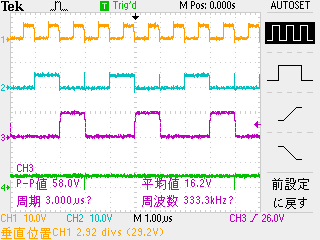
\includegraphics[width=0.4\textwidth]{assets/hidouki.png}
  \caption{CLK、\(Q_0\)、\(Q_1\)、CLRの観測波形}
\end{figure}

また、図4.16より作成した非同期式1/3カウンタのタイミングチャートを図4.17に示す。

\begin{figure}[H]
  \centering
  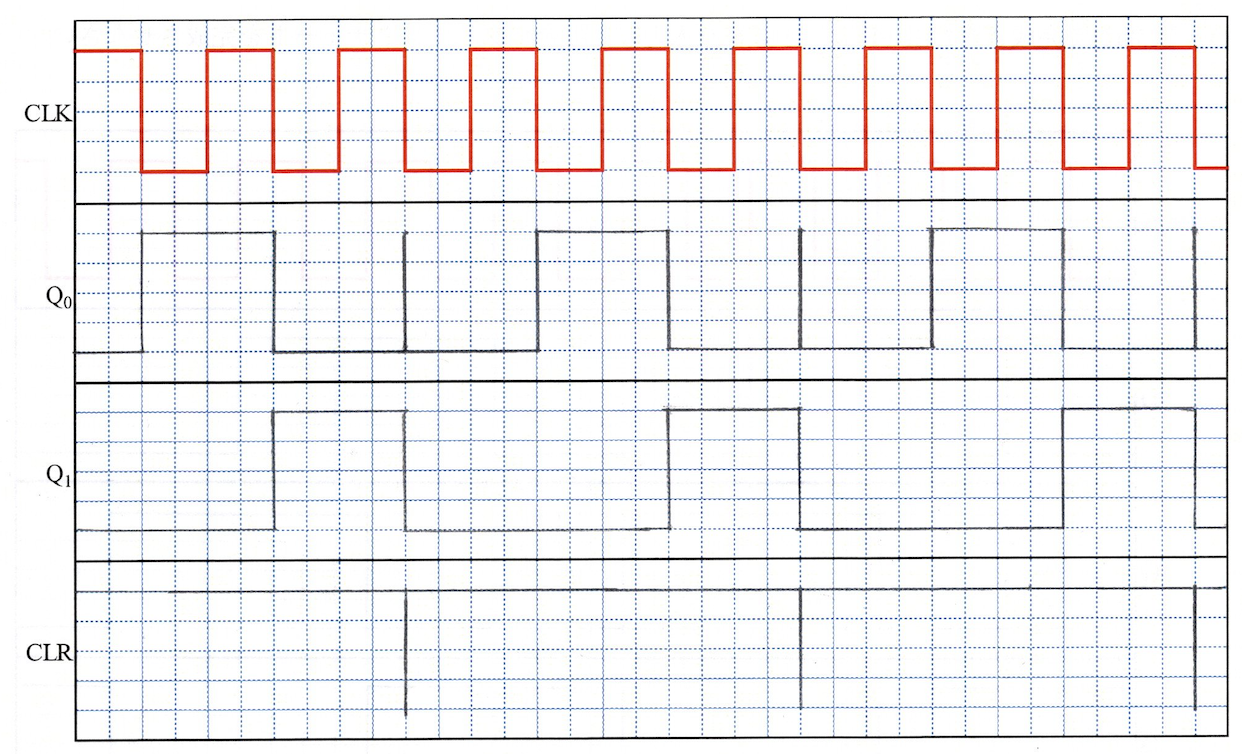
\includegraphics[width=0.8\textwidth]{assets/hidoukichart.png}
  \caption{非同期式1/3カウンタのタイミングチャート}
\end{figure}

図4.17より、Q0がクロックの立ち上がりで反転し、Q1はQ0の立ち上がりに応じて反転していることがわかる。

\subsubsection{同期式1/3カウンタ}
図3.7の回路を制作し、各測定点(CLK, 1J, \(Q_0\), \(Q_1\))のオスロスコープで観測した波形を図4.18(上から順にCLK、1J、Q0, Q1)に示す。

\begin{figure}[H]
  \centering
  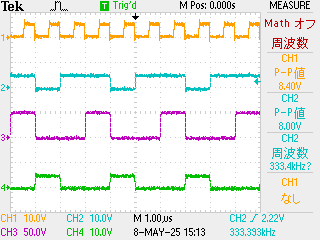
\includegraphics[width=0.4\textwidth]{assets/douki.png}
  \caption{CLK、1J、\(Q_0\), \(Q_1\)の観測波形}
\end{figure}

また、図4.18より作成した同期式1/3カウンタのタイミングチャートを図4.19に示す。

\begin{figure}[H]
  \centering
  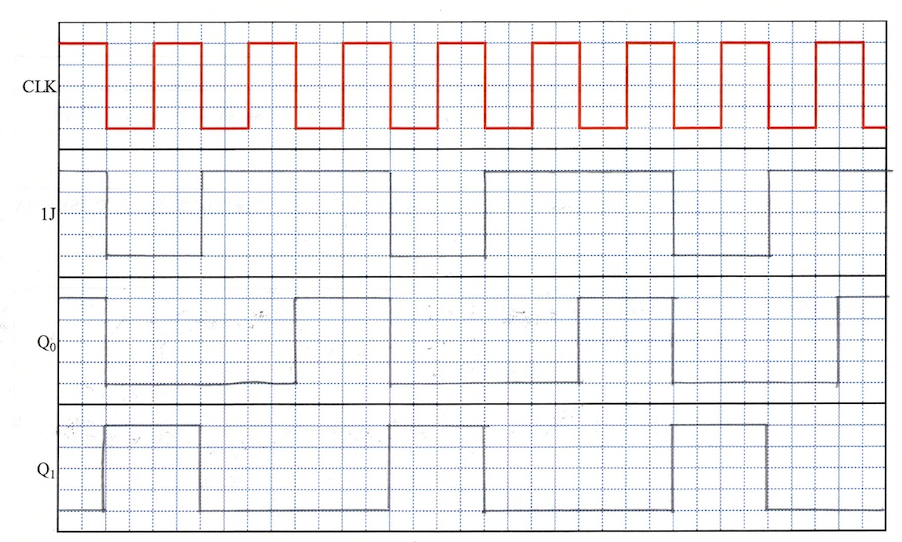
\includegraphics[width=0.8\textwidth]{assets/doukichart.png}
  \caption{同期式1/3カウンタのタイミングチャート}
\end{figure}

図4.19より、1J,Q0,Q1はそれぞれCLKの3倍周期で規則的に変化していることが確認できる。

\subsection{メモリ機能}
図3.7の回路を作成し、表3.1の操作を実施した結果を以下に示す。
\begin{enumerate}
  \item WRITE=0, CTRL=1, ワード線=1 の場合
  \begin{itemize}
    \item 2SK679Aのドレインにかかる電圧:0.00V
    \item ゲートにかかる電圧:5.03V
    \item 状態:オフ状態
  \end{itemize}
  \item WRITE=1, CTRL=1, ワード線=1 の場合
  \begin{itemize}
    \item 2SK679Aのドレインにかかる電圧:5.03V
    \item ゲートにかかる電圧:5.03V
    \item A点の電圧:3.92V
    \item 理由:ドレインにかかる電圧が5.03Vであるため、2SK679Aはオン状態となり、他の素子に分圧され、A点の電圧は下がる。
    \item 読み出し操作をしたときのB点の電圧:5.03V
  \end{itemize}
\end{enumerate}

\section{考察}

\subsection{半加算器(HA)}
\subsubsection{ド・モルガンの法則についての説明}
ド・モルガンの法則は、以下の2式で表される。
\begin{equation}
  \overline{A \cdot B} = \overline{A} + \overline{B}
\end{equation}
\begin{equation}
  \overline{A + B} = \overline{A} \cdot \overline{B}
\end{equation}
今回の実験では、ド・モルガンの法則を用いて、NOTゲートとNANDゲートを使用したORゲートの構成と、NOTゲートとNORゲートを使用したANDゲートの構成を確認した。これにより、ド・モルガンの法則が成り立つことが実験的に確認できた。

\subsubsection{ド・モルガンの法則が成り立つメリット}
ド・モルガンの法則が成り立つことで、論理式の簡略化や、論理回路の設計が容易になる。特に、ディジタル回路の設計においてはは、NANDゲートやNORゲートを用いて他のゲートを構成することで、部品数を節約し、回路の集積度を高めることができる。これにより、回路のコスト削減や、動作速度の向上が期待できる。

\subsubsection{全加算機(FA)と半加算器(HA)の動作・真理値表の記載}
半加算器は、2つの入力信号AとBを持ち、出力は和SとキャリーCである。半加算器の動作は以下の論理式で表される:
\begin{align}
  S &= A \oplus B \\
  C &= A \cdot B
\end{align}
ここで、\(\oplus\)はXOR(排他的論理和)、\(\cdot\)はAND(論理積)を表す。

半加算器の真理値表は以下の表5.1のようになる。
\begin{table}[H]
  \centering
  \caption{半加算器の真理値表}
  \begin{tabular}{|c|c|c|c|}
    \hline
    A & B & S & C \\ \hline
    0 & 0 & 0 & 0 \\ \hline
    0 & 1 & 1 & 0 \\ \hline
    1 & 0 & 1 & 0 \\ \hline
    1 & 1 & 0 & 1 \\ \hline
  \end{tabular}
\end{table}

全加算器は、2つの入力信号AとBに加えて、前回の計算結果を表すキャリー入力Cを持つ。全加算器の出力は、和Sとキャリー出力Coutである。全加算器の真理値表は以下の表5.2ようになる。
\begin{table}[H]
  \centering
  \caption{全加算器の真理値表}
  \begin{tabular}{|c|c|c|c|c|}
    \hline
    A & B & C & S & Cout \\ \hline
    0 & 0 & 0 & 0 & 0 \\ \hline
    0 & 0 & 1 & 1 & 0 \\ \hline
    0 & 1 & 0 & 1 & 0 \\ \hline
    0 & 1 & 1 & 0 & 1 \\ \hline
    1 & 0 & 0 & 1 & 0 \\ \hline
    1 & 0 & 1 & 0 & 1 \\ \hline
    1 & 1 & 0 & 0 & 1 \\ \hline
    1 & 1 & 1 & 1 & 1 \\ \hline
  \end{tabular}
\end{table}

全加算器は、2つの半加算器と1つのORゲートを組み合わせて構成される。最初の半加算器は入力AとBを受け取り、和S1とキャリー出力C1を生成する。次に、S1とキャリー入力Cを2つ目の半加算器に入力し、最終的な和Sとキャリー出力C2を生成する。最後に、C1とC2をORゲートに入力して最終的なキャリー出力Coutを得る。

全加算器の動作を数式で表すと以下のようになる。
\begin{align}
  S1 &= A \oplus B \\
  C1 &= A \cdot B \\
  S &= S1 \oplus C \\
  C2 &= S1 \cdot C \\
  Cout &= C1 + C2
\end{align}

全加算器の真理値表は以下の表5.3のようになる:
\begin{table}[H]
  \centering
  \caption{全加算器の真理値表}
  \begin{tabular}{|c|c|c|c|c|}
    \hline
    A & B & C & S & Cout \\ \hline
    0 & 0 & 0 & 0 & 0 \\ \hline
    0 & 0 & 1 & 1 & 0 \\ \hline
    0 & 1 & 0 & 1 & 0 \\ \hline
    0 & 1 & 1 & 0 & 1 \\ \hline
    1 & 0 & 0 & 1 & 0 \\ \hline
    1 & 0 & 1 & 0 & 1 \\ \hline
    1 & 1 & 0 & 0 & 1 \\ \hline
    1 & 1 & 1 & 1 & 1 \\ \hline
  \end{tabular}
\end{table}

このように、全加算器は2つの半加算器と1つのORゲートを用いることで、3つの入力信号(A, B, C)に対して和Sとキャリー出力Coutを計算することができる。

\subsubsection{キャリールックアヘッドに関して}

キャリールックアヘッド回路とは、加算回路において各桁のキャリー(繰り上がり)を下位の計算結果を待たずに、入力値から直接計算する仕組みである。各ビットの入力$a_i, b_i$から「生成(generate)」$g_i = a_i b_i$および「伝搬(propagate)」$p_i = a_i \oplus b_i$を求め、これらを用いて各桁のキャリー$C_i$を論理式で一括して計算する。例えば4ビットの場合、キャリーは次式のように表される。
\begin{align*}
C_1 &= g_0 + p_0 C_0 \\
C_2 &= g_1 + p_1 g_0 + p_1 p_0 C_0 \\
C_3 &= g_2 + p_2 g_1 + p_2 p_1 g_0 + p_2 p_1 p_0 C_0 \\
C_4 &= g_3 + p_3 g_2 + p_3 p_2 g_1 + p_3 p_2 p_1 g_0 + p_3 p_2 p_1 p_0 C_0
\end{align*}
このように、各桁のキャリーを下位桁の入力値から直接求めることで、キャリー伝搬による遅延を大幅に削減することができる。実際の回路設計では、論理ゲートの入力数(ファンイン)制限を考慮し、4ビット単位などで階層的に実装される。

\subsection{信号発生器の設計と作成}
\subsubsection{信号発生器(SG)からディジタル波形が生じる流れについて}
信号発生器は、アナログ信号を0と1のディジタル信号に変換するための装置である。タイミングチャートより、A点の正弦波が0Vを閾値として、NOTゲートがHIGHとLOWを判定し、出力信号を反転させアナログ信号をディジタル信号に変換して出力していることがわかる。またNOTゲートを直列に繋ぐことで、もとの正弦波と位相を合わせている。\\
1つ目のJK-FFによってCLK信号をQ1と\(\overline{Q1}\)に分け、周期を2倍にしており、2つ目のJK-FFによってQ1信号をSとRに分け、周期をさらに2倍にしている。これにより、最終的にSとRの信号はCLK信号の4倍の周期となる。

\subsubsection{部品($50\,\Omega$、$0.1\,\mathrm{\mu F}$、$470\,\mathrm{\mu F}$)の名称と役割についての説明}
$50\,\Omega$抵抗は信号発生回路のインピーダンス整合に用いられている。$0.1\,\mathrm{\mu F}$コンデンサは高周波信号に対するバイパスコンデンサとして機能している。$470\,\mathrm{\mu F}$コンデンサは、電源からの信号をフィルタリングし、安定した出力信号を得るために使用されている。さらに低周波信号に対するバイパスコンデンサとしても機能している。

\subsection{同期式SR-FFの動作と特性}
\subsubsection{同期式SR-FFの動作についての説明}
同期式SR-FF(Set-Resetフリップフロップ)は、2つの入力(S: Set, R: Reset)によって出力Qとその反転$\overline{Q}$を制御する記憶素子である。今回はNANDゲートを用いて構成した。真理値表を表5.4に示す。

\begin{table}[H]
  \centering
  \caption{同期式SR-FFの真理値表}
  \begin{tabular}{|c|c|c|c|}
    \hline
    S & R & Q(next) & 備考 \\ \hline
    1 & 0 & 1 & セット状態 \\ \hline
    0 & 1 & 0 & リセット状態 \\ \hline
    1 & 1 & Q & 無変化(保持) \\ \hline
    0 & 0 & 不定 & 禁止状態 \\ \hline
  \end{tabular}
\end{table}

このように、同期式SR-FFは入力SとRの組み合わせによって出力状態を制御し、記憶素子として機能する。ただし、SとRが同時に0になる禁止状態は避ける必要があるため、実際の回路設計ではこの状態が発生しないように工夫される。

図4.10より、SとQの位相が1クロック分ずれていることが確認できる。また、Rと$\overline{Q}$の位相も1クロック分ずれていることが確認できる。
これは、今回実験で用いたSR-FFがクロック同期式であることと合致する。

\subsubsection{エッジトリガについて}
図5.2のタイミングチャートより、表5.4の真理値表のとおり、CLKの立ち上がりエッジでSとRの状態に応じて出力Qと$\overline{Q}$が変化することが確認できた。

\subsection{JK-FFの動作と特性}
表2.4の真理値表より、初期状態が0かつJ=1となったとき(今回の実験では常にK=1)、次のCLKの立ち下がりエッジでQが1に変化することが確認できた。初期状態が1かつJ=1となった次の立ち下がりエッジで、Qが0となることも確認することができた。

\subsection{D-FFの動作と特性}
図4.15より、DとQの位相が1クロック分ずれていることが確認できる。これは表4.6の真理値表とも合致し、さらにCLK信号の立ち下がりエッジでDの状態に応じて出力されていることも確認できた。

\subsection{1/3カウンタ}
\subsubsection{非同期式でハザードが出るメカニズムと同期式の動作の説明}
図4.17より、Q0とQ1が3通りの状態(00→01→10)を順に繰り返していることが確認できる。また、CLR信号がLOWになると、即座にQ0とQ1の出力が00にリセットされる動作が確認できる。\\

図3.5より、CLR信号はQ0とQ1のNAND出力となっていることがわかる。したがって、Q0とQ1の出力が11のとき、CLR信号はLOWとなりQ0とQ1はリセットされる。しかし、Q0とQ1の出力が00に戻されるまでには数十ns程度の時間がかかるため、CLR信号がLOWの状態が数十ns続くことになる。このごく短い出力がハザードとして観測できると考えられる。\\

Q0とQ1が3通りの状態(00→01→10)を順に繰り返していることが確認できる。また、カウントはCLKの立ち下がりエッジで行われていることがわかる。

\subsubsection{非同期、同期カウンタのメリットとデメリットについて}
\begin{enumerate}
  \item 非同期カウンタ
  \begin{enumerate}
    \item メリット \\
    ・クロック配線がシンプルで、回路規模が小さい場合は構成が簡単である。\\
    ・フリップフロップ同士を直列につなぐだけでカウンタが構成できるため、回路規模が小さくできる。\\
    \item デメリット \\
    ・各フリップフロップにクロックが順次伝播するため、回路内でクロック遅延が発生しやすい。\\
    ・動作周波数が高くなると遅延が大きくなり、タイミング不良や「すっぽ抜け」などの問題が発生しやすい。\\
    ・外部要因による遅延変動の影響を受けやすく、実機での動作が不安定になることがある。\\
  \end{enumerate}
   \item 同期カウンタ
  \begin{enumerate}
    \item メリット \\
    ・全てのフリップフロップが同一クロックの同一エッジで動作するため、タイミングが揃いやすく、設計の信頼性が高い。\\
    ・クロック・スキュー(クロックの到達時間のズレ)が最小になるように調整されるため、データの「すっぽ抜け」や競合などの問題が起こりにくい。\\
    ・外部要因(電圧変動、温度変化など)による遅延の影響を受けにくく、実機での動作が安定しやすい。
    \item デメリット \\
    ・複雑な回路や大規模なデバイスでは、クロック配線が増えて設計や配線が複雑になりやすい。\\
    ・クロック配線の負荷が大きくなり、消費電力が増える場合がある。
  \end{enumerate}
\end{enumerate}

以上の理由より、信頼性・安定性が重要な場合は同期カウンタが推奨される。回路規模が小さく、シンプルさを優先する場合は非同期カウンタも選択肢となるが、高速動作や大規模回路では同期設計が基本となる。

\subsection{メモリ機能}

\subsubsection{DRAM回路の動作説明}

DRAMでは、コンデンサに電荷が溜まっている状態を"1"、溜まっていない状態を"0"としてデータを記憶している。\\
書き込みは、ワード線の電圧を上げた状態で行い、"1"の書き込み時には、データ線の電圧を上げる。これによりトランジスタがオンになりコンデンサが充電される。"0"の書き込み時には、データ線の電圧を下げることでコンデンサが放電される。\\
読み出しは、ワード線の電圧を上げることで、トランジスタをONにする。データ線の電位の変化が瞬間的に変化すれば"1"が読み出せ、変化しなければ"0"が読み出せる。 \\

\subsubsection{書き込み時の電圧が4V程度になる理由}
トランジスタがオンの状態では、ドレインからソースへの電流が流れる。図5.1のデータシートより、トランジスタのドレイン・ソース間のオン抵抗 $R_{\text{DS(on)}}$ は最大で1Ω程度(条件:$V_{GS}=4V, I_D=0.5A$)である。\\
書き込み時、すなわちMOSFETのオン状態ではオン抵抗があるために、電流が流れるときに電圧降下が発生し、ソース側の電圧が下がるためであると考えられる。

\begin{figure}[H]
  \centering
  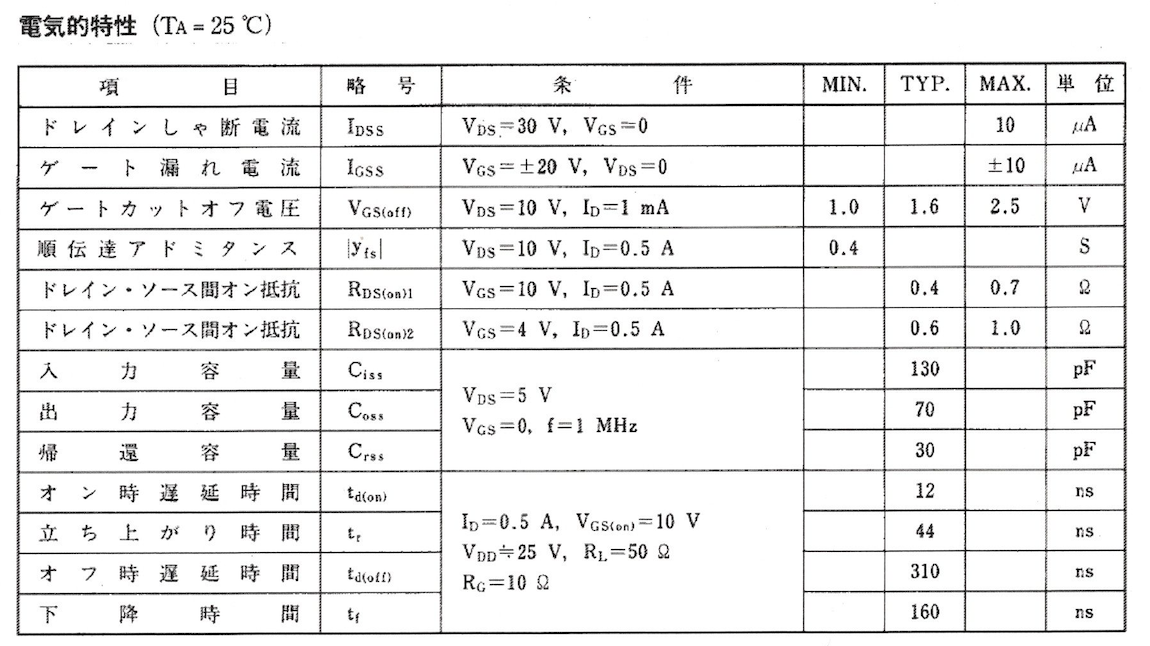
\includegraphics[width=0.8\textwidth]{assets/datasheet.png}
  \caption{2SK679Aのデータシート}
\end{figure}

\subsubsection{読み出し時に電圧が5Vになる理由}
今回の実験では、書き込み時に"1"を記録したため、データ線に5Vが出力され、表5.5のTC74HC126の真理値表より、HIGHを出力したためだと考えられる。

\begin{table}[H]
  \centering
  \caption{TC74HC126の真理値表}
  \begin{tabular}{c}
    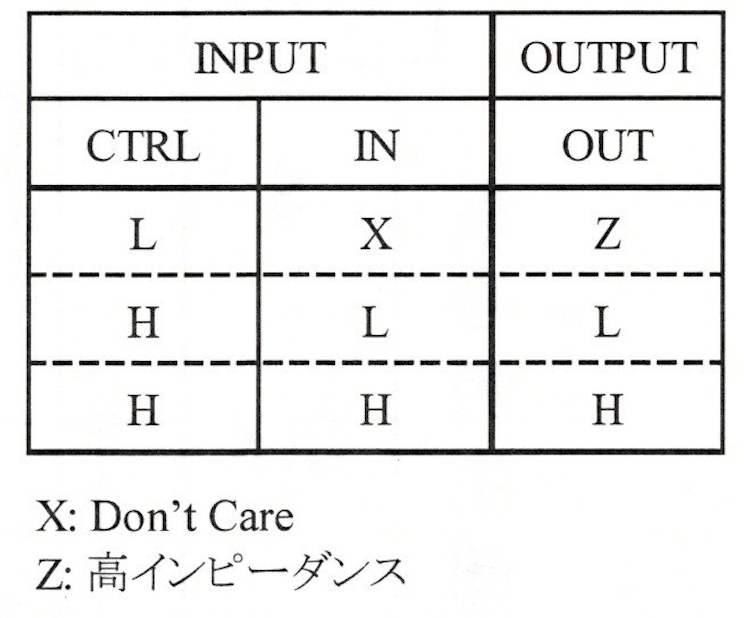
\includegraphics[width=0.3\textwidth]{assets/tc74hc126shinri.png} \\
  \end{tabular}
\end{table}

\subsubsection{DRAMとSRAMの比較}
DRAMとSRAMの違いを表5.6に示す。

\begin{table}[H]
  \centering
  \caption{DRAMとSRAMの比較}
  \begin{tabular}{|l|l|l|}
    \hline
    項目 & \textbf{DRAM(Dynamic RAM)} & \textbf{SRAM(Static RAM)} \\ \hline
    記憶方式 & トランジスタ+キャパシタ(電荷で記憶) & フリップフロップ回路(トランジスタ6個) \\ \hline
    リフレッシュ & 必要(定期的に電荷を補充) & 不要(電源供給中はデータ保持) \\ \hline
    アクセス速度 & 遅め(リフレッシュの影響) & 非常に速い \\ \hline
    集積度 & 高い(構造がシンプル) & 低い(構造が複雑) \\ \hline
    消費電力 & 比較的高い(常にリフレッシュ) & 待機時は低い、アクセス時は高くなる場合あり \\ \hline
    コスト & 安価(大容量でも低コスト) & 高価(1ビットに6トランジスタ) \\ \hline
    主な用途 & メインメモリ(RAM) & キャッシュメモリ、レジスタなど \\ \hline
  \end{tabular}
\end{table}

DRAMはキャパシタに電荷を蓄えることで情報を記憶するが、電荷が自然放電するため定期的なリフレッシュが必要である。その分アクセス速度はSRAMに劣る。その代わり、構造がシンプルなため大量のメモリを安価に実装できる。\\
SRAMはトランジスタのみで構成されるフリップフロップ回路で情報を保持し、リフレッシュ不要で高速アクセスが可能である。ただし、構造が複雑で面積あたりの記憶容量が少なく、高コストとなる。

\section{使用機材}
表6.1に示す。
\begin{table}[H]
  \centering
  \caption{使用機材一覧}
  \begin{tabular}{|c|c|c|c|}
    \hline
    名称 & 型式 & 製造元 & 管理番号 \\ \hline
    直流電流源 & PMC35-1.2DU & KIKUSUI & UK002986 \\ \hline
    ファンクションジェネレータ & FG-274 & TEXIO & 17073061 \\ \hline
    オシロスコープ & TDS 2004B & Tektronix & C100578 \\ \hline
    デジタルマルチメータ & CD731 & Sanwa & 0152985 \\ \hline
  \end{tabular}
\end{table}

\section{参考文献}
\begin{enumerate}
\item 「CMOSとは?NOTゲートの動作原理をもとに解説」, \\
\url{https://ushitora.net/archives/546}, \\
閲覧日: 2025年5月12日
\item 「CMOSロジック回路の基礎(第2章2節)」, 東芝デバイス&ストレージ株式会社, \\
\url{https://toshiba.semicon-storage.com/jp/semiconductor/knowledge/e-learning/cmos-logic-basics/chap2/chap2-2.html}, \
閲覧日: 2025年5月12日
\item 「TC74HC107AP/AF データシート」, matrutsu, \\
\url{https://www.marutsu.co.jp/contents/shop/marutsu/datasheet/74HC107.pdf}, \\
閲覧日: 2025年5月12日
\item 「15. フリップフロップ」, CTLEEC, \\
\url{http://www.ctleec.sakura.ne.jp/2024/01/31/15-フリップフロップ/ }, \\
閲覧日: 2025年5月12日
\item 「半加算器(1bit加算器)の回路図と動作原理, 知能デバイス研究所, \\
\url{https://ushitora.net/archives/570}, \\
閲覧日: 2025年5月12日
\item 全加算器(n bit加算器)の回路図と動作原理, 知能デバイス研究所, \\
\url{https://ushitora.net/archives/588}, \\
閲覧日: 2025年5月12日
\item フリップフロップ回路とは? ラッチとの違いや種類別の基本構造・動作原理・使用例を解説 \\
\url{https://tonarism.co.jp/media/media_detail.php?b_id=72}, \\
閲覧日: 2025年5月12日
\item Ques10 Draw the circuit of JK FF using NAND gates and write the truth table, \\
\url{https://www.ques10.com/p/14914/draw-the-circuit-of-jk-ff-using-nand-gates-and-wri/}, \\
閲覧日: 2025年5月13日
\item 桁上げ先見加算器、保存加算器の性質, 電気情報の森, \\
\url{https://denjoforest.com/full-adder}, \\
閲覧日: 2025年5月13日\
\item RTL 設計ビギナー必見 同期設計と非同期設計の違い, マクニカ, \\
\url{https://www.macnica.co.jp/business/semiconductor/articles/intel/119381/}, \\
閲覧日: 2025年5月13日
\item 同期式回路と非同期式回路の違い~結論編~, マクニカ, \\
\url{https://www.macnica.co.jp/business/semiconductor/articles/intel/133451/ }, \\
閲覧日: 2025年5月13日
\item DRAMとは:構造と動作原理, セミジャーナル, \\
\url{https://semi-journal.jp/basics/device/memory/dram-structure.html}, \\
閲覧日: 2025年5月13日
\item DRAMとSRAMの違いは? それぞれの仕組み・特徴・用途を比較, トナリズム, \\
\url{https://tonarism.co.jp/media/media_detail.php?b_id=33}, \\
閲覧日: 2025年5月13日
\end{enumerate}

\end{document}